\chapter{Experimental Apparatus}
\label{ch:experiment}

As this thesis is focused on the physics of heavy-ion collisions, it stands to reason that the data analyzed in this thesis was gathered using the only detector along the LHC dedicated to studying such collisions: the ALICE detector. In this chapter, a brief synopsis of the LHC will be provided, followed by a much more detailed overview of the ALICE detector and its sub-detectors most relevant to this thesis.

\section{The LHC}
Located along the Swiss-French border near Geneva, Switzerland, the Large Hadron Collider (LHC)~\cite{LHC1, LHC2} is the largest particle accelerator on the planet. At a circumference of 27 kilometers, its tunnels lie almost 200 meters beneath the surface of the earth. Inside the tunnels are two high-energy particle beams pointing in opposite directions, with the beam pipes being kept inside of an ultra-high vacuum.
The particles inside the beam are guided by a multitude of superconducting magnets: 393 quadrupole magnets keep the beam focused, while 1232 dipole magnets bend the particles along the circular path. 
The beams are designed to collide at four intersection points along the LHC, each with a corresponding detector surrounding the collision points: 
\begin{enumerate}
\item ALICE~\cite{ALICE}, designed for investigating heavy-ion collisions
\item ATLAS~\cite{ATLAS}, designed for studying high-$p_{T}$ particles produced in pp collisions 
\item CMS~\cite{CMS},   designed for precise detection of muons
\item LHCb~\cite{LHCb}, designed for studying CP violations through measurements of B mesons at forward rapidity
\end{enumerate}
Note that ``designed for'' does not mean that these detectors are incapable of investigating other facets of particle collisions. For example, the ALICE detector is plenty capable for studying pp collisions\cite{ALICEpp1, ALICEpp2}, and the ATLAS and CMS detectors have been used to publish exciting results for heavy-ion collisions~\cite{CMSHeavy1, ATLASHeavy1}. A diagram of the LHC with these four intersection points can be seen in Figure \ref{fig:lhcring}.
\begin{figure}
    \centering
    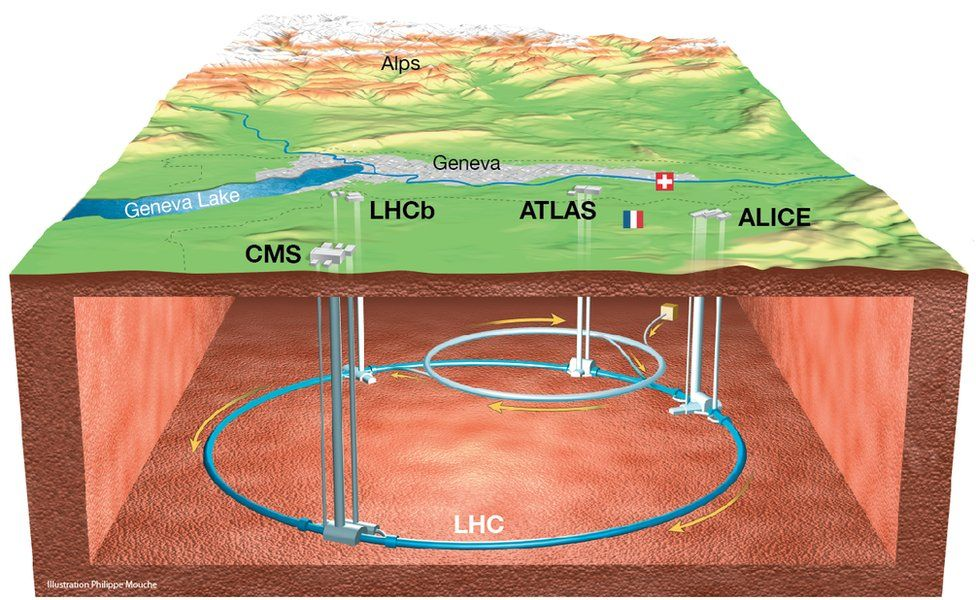
\includegraphics[width=0.8\textwidth]{figures/experiment/lhcring_illustration.jpeg}
    \caption{A diagram depicting the LHC with its various main detectors shown underground. Illustration by Philippe Mouche, taken from~\cite{LHCBBC}}
    \label{fig:lhcring}
\end{figure}
As of 2023, the highest center of mass energies achieved for each of the main collision systems (pp, p--Pb, Pb--Pb) are $\sqrt{s}$ = 13.6 TeV for pp, $\sqrt{s}$ = 7 TeV for p-Pb and $\sqrt{s}$ = 5.36 TeV for Pb--Pb. 

\section{The ALICE Detector}
The detector used by the A Large Ion Collider Experiment (ALICE) collaboration, unsurprisingly known as the ALICE detector, has the primary focus of investigating the physical properties of the strongly interacting quark-gluon plasma created during heavy-ion collisions.
Building the detector was a massive effort, requiring the help from over 1000 people from 105 institutes in 30 different countries. 
The detector itself is also massive, weighing in at around 10,000 tons, and spanning 26 meters in length with a 16-meter height and width.
It is composed of 18 sub-detector systems, all of which work together to help reconstruct the event.
A diagram of the detector with its corresponding sub-detector systems can be seen in Figure \ref{fig:alice_detector}.
\begin{figure}
    \centering
    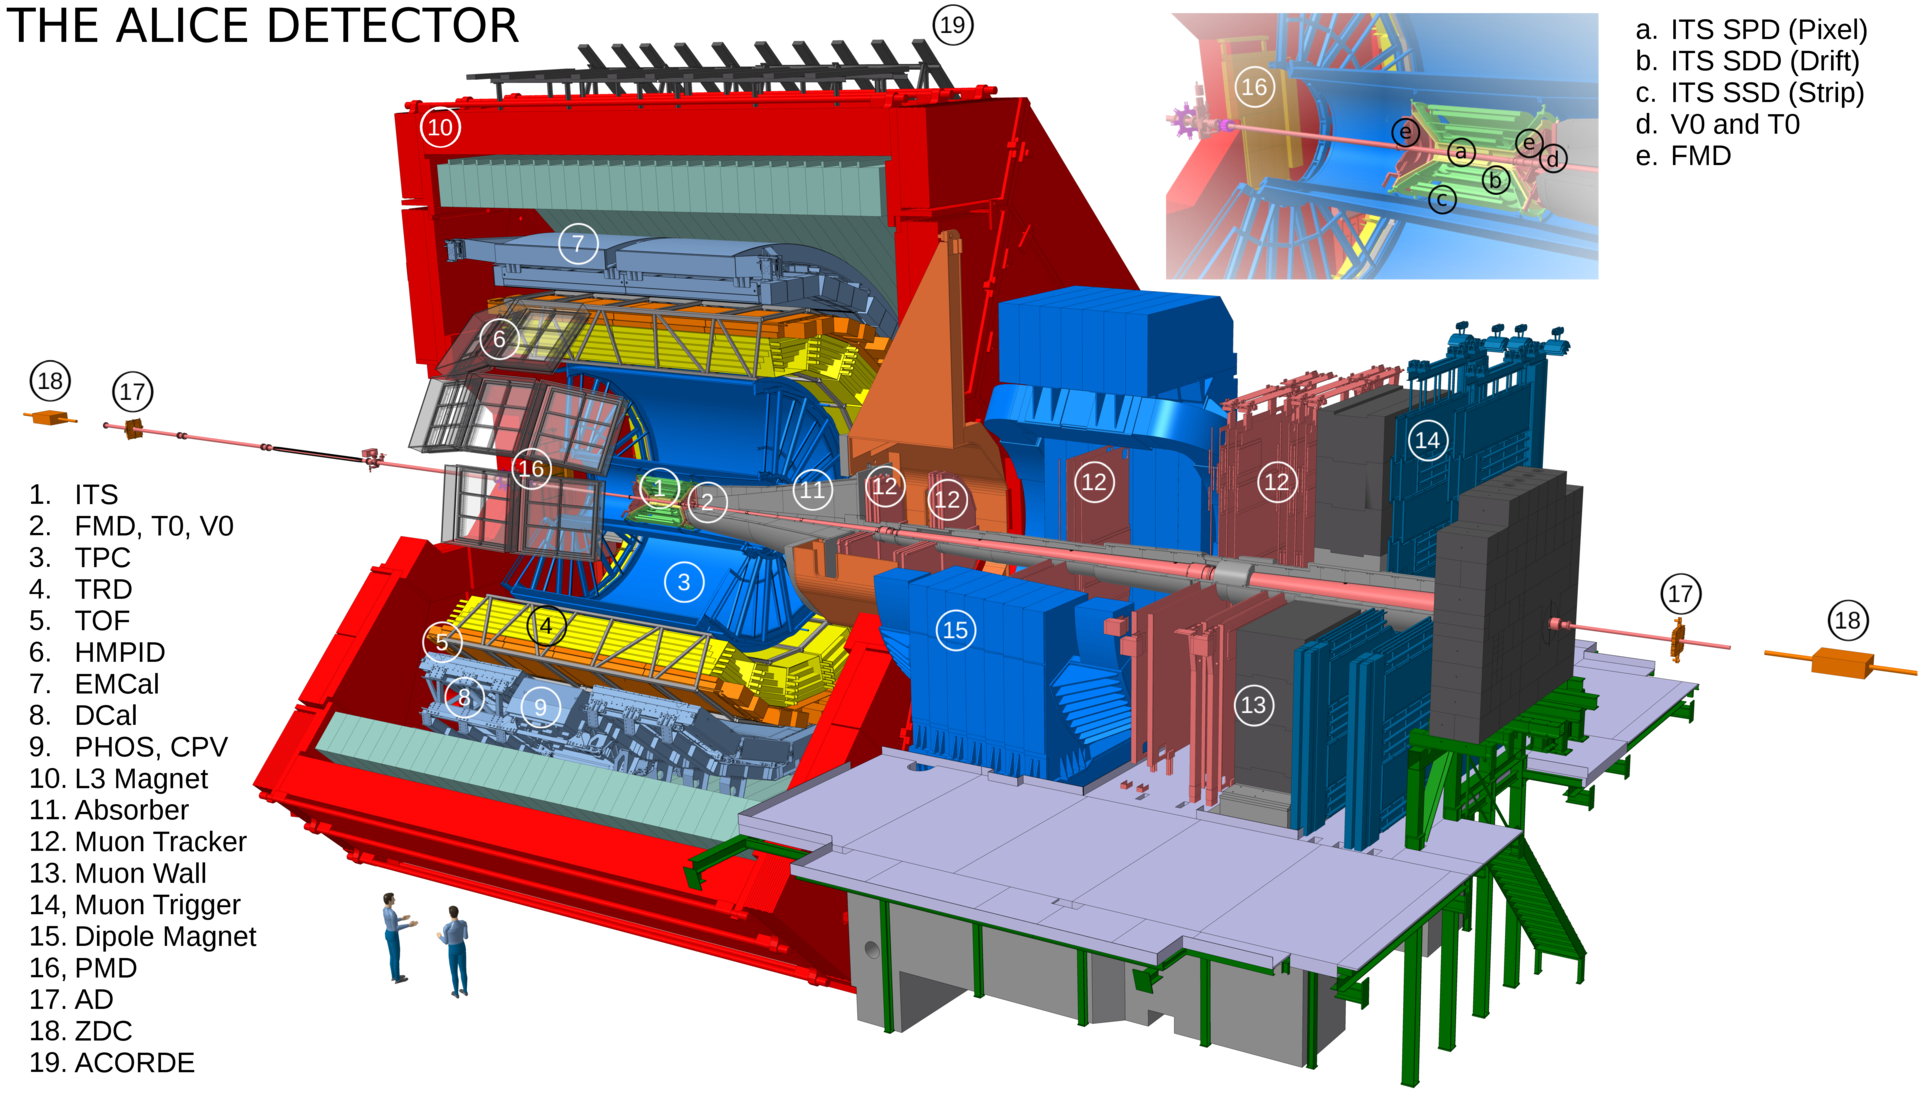
\includegraphics[width=0.8\textwidth]{figures/experiment/ALICE_detector_schematic.png}
    \caption{A 3-D schematic of the ALICE detector, with labels for all of the sub-detectors, taken from~\cite{ALICEDiagram}. Note the humans-for-scale in the bottom left of the diagram.}
    \label{fig:alice_detector}
\end{figure}
As the primary focus of the ALICE detector is to study heavy-ion collisions, all of its components must work together to reconstruct very high multiplicity events. The components most relevant to this thesis will be discussed in the following sections.

\subsection{Detector coordinates}
Before discussing the components of the ALICE detector, it is important to first define a coordinate system suitable for describing the geometry of the detector and the collisions within. As the ALICE detector is a giant cylinder, the most pragmatuc choice is cylindrical coordinates, with the $z$-axis pointing along the beam line. An example of this cylindrical coordinate system is shown in Figure \ref{fig:detector coordinates}. The plane defined by the x- and y-axes is often referred to as the \textbf{transverse plane}, with the angle $\varphi$ referred to as the \textbf{azimuthal angle}.

\begin{figure}
    \centering
    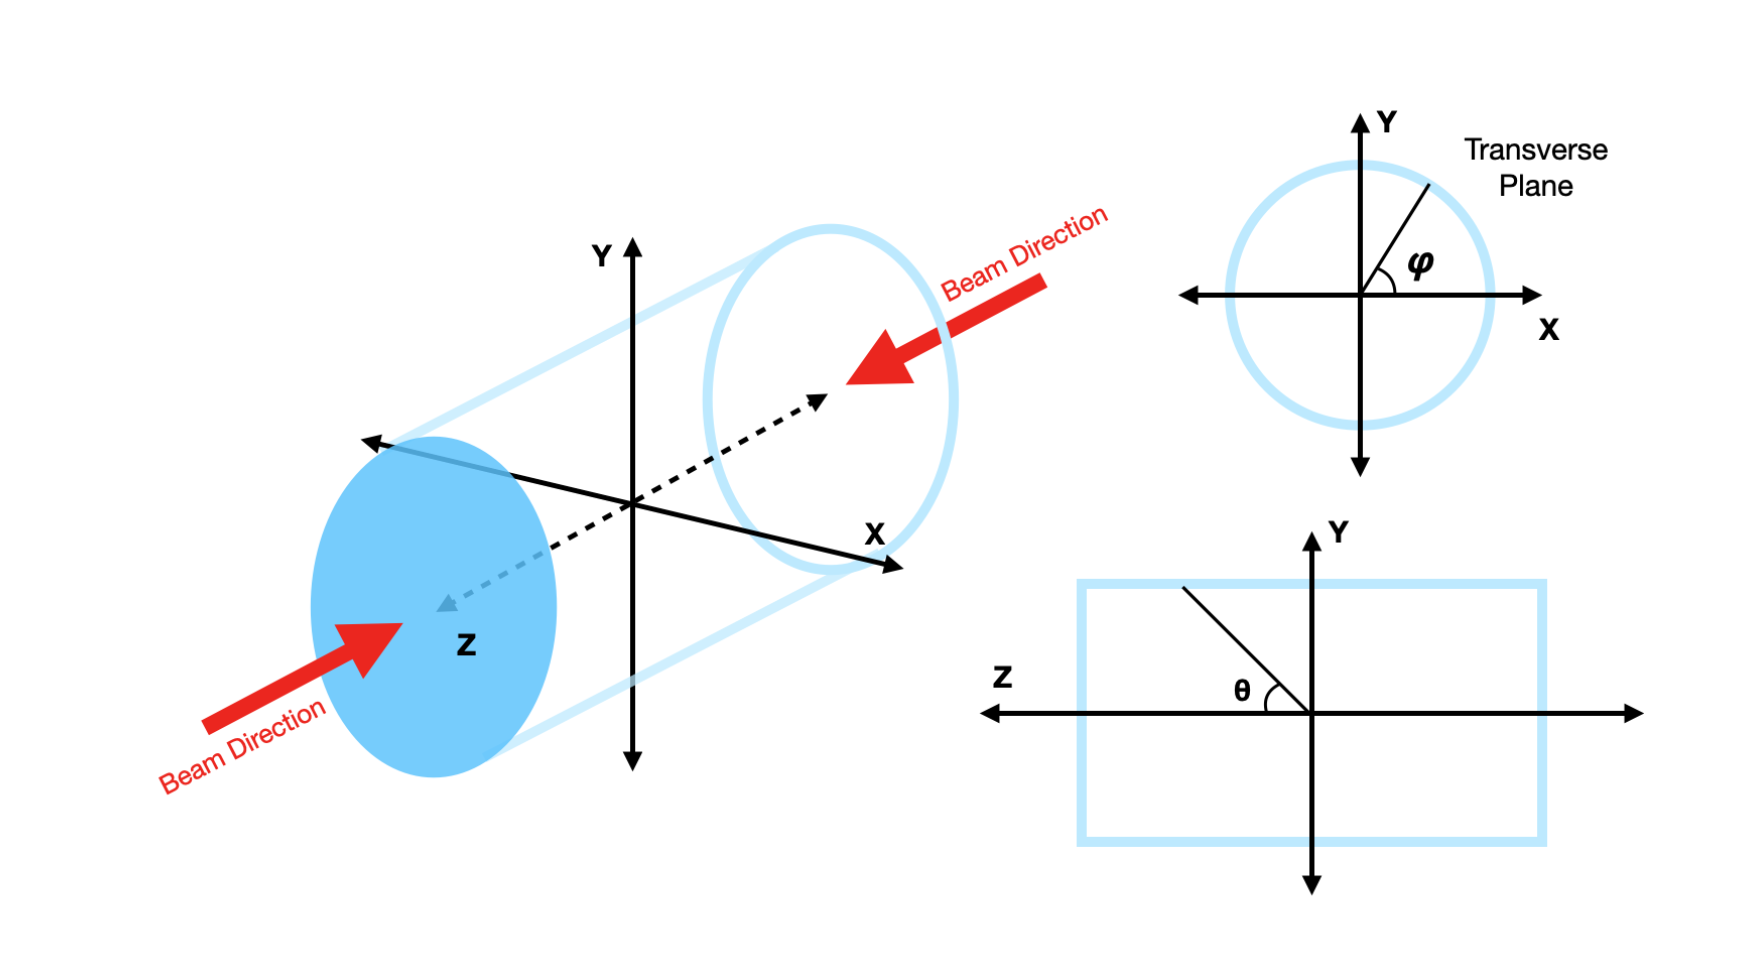
\includegraphics[width=0.8\textwidth]{figures/experiment/detector_coordinates.png}
    \caption{A diagram showing the cylindrical coordinate system used to describe the ALICE detector.}
    \label{fig:detector coordinates}
\end{figure}

Unfortunately, collisions within the ALICE detector involve particles moving at relativistic speeds in the beam (z) direction. Thus the polar angle $\theta$ is not particularly useful, as it is not Lorentz invariant. Instead, a more useful quantity is the rapidity $y$, which can be defined as
\begin{equation}
    y = \frac{1}{2} \ln \left( \frac{E + p_{z}}{E - p_{z}} \right),
\end{equation}
where $E$ is the energy of the thing being measured and $p_{z}$ is the momentum in the z-direction. This quantity is preferable to $\theta$ as differences in rapidity are invariant under Lorentz boosts along the z-axis. This follows directly from the fact that rapidity is often defined in terms of such boosts,
\begin{equation}
    \left(\begin{array}{c}
        c t^{\prime} \\
        z^{\prime}
        \end{array}\right)=\left(\begin{array}{cc}
        \cosh y & -\sinh y \\
        -\sinh y & \cosh y
        \end{array}\right)\left(\begin{array}{c}
        c t \\
        z
        \end{array}\right) \equiv \Lambda(y)\left(\begin{array}{c}
        c t \\
        z
        \end{array}\right).
\end{equation}
It can be shown\footnote{Using various properties of the hyperbolic trigonometric functions.} that $\Lambda(y)$ obeys
\begin{equation}
    \Lambda(y_1 + y_2) = \Lambda(y_1)\Lambda(y_2),
\end{equation}
which in turn gives a rapidity addition rule for reference frames A, B and C moving along the z-axis,
\begin{equation}
    y_{AC} = y_{AB} + y_{BC}.
\end{equation}
Now suppose reference frame A is the lab (stationary) frame, and reference frames B and C correspond to two different particles. The above equation can then be written as
\begin{equation}
    y_{AC} - y_{AB} = y_{BC} = y_{A'B} - y_{A'C},
\end{equation}
where $A'$ can be \textit{any} reference frame. In other words, the difference in rapidity between any two particles does not depend on the reference frame the measurement is made in. Another consequence of this property is that rapidity distributions of particles do not change shape in different reference frames: they only get shifted along the rapidity axis.

However, the total energy of a given particle is often not known, and thus rapidity is replaced by the more experiment-friendly \textbf{pseudorapidity}, 
\begin{equation}
    \eta = \frac{1}{2} \ln \left( \frac{|\vec{p}| + p_{z}}{|\vec{p}| - p_{z}} \right) 
        = -\ln \left( \tan \frac{\theta}{2} \right),
\end{equation}
where $\theta$ is the aforementioned polar angle. This quantity can be directly measured by experiment, at the expense of losing a small amount of Lorentz invariance: the \textit{pseudo} part of pseudorapidity comes from the idea that at very high momentum ($p >> m$), the rapidity and pseudorapidity are approximately equal.

\section{The Inner Tracking System}
\label{sec:its}

The Inner Tracking System (ITS)~\cite{ITS} is the inner most component of the ALICE detector, lying closest to the beam pipe. It is composed of six cylindrical layers of silicon detectors that are coaxial with the beam pipe and cover the pseudorapidity range $|\eta| \leq 0.9$. The distance from the beam line varies from 3.9 cm for the first layer to 43 cm for the sixth layer. A diagram of the ITS can be seen in Figure~\ref{fig:its_schematic}. Because of its proximity to the interaction point, the ITS is invaluable for reconstructing both primary and secondary vertices and enhancing the tracking capabilities of the ALICE detector near the interaction point. Moreover, the ITS can also track particles that are not detected or missed by the external barrel detector due to acceptance limitations and momentum cutoff. 

\begin{figure}
    \centering
    \includegraphics[width=0.8\textwidth]{figures/experiment/its_diagram.png}
    \caption{A schematic of the ITS showing the six layers of silicon detectors, taken from~\cite{ITSDiagram}.}
    \label{fig:its_schematic}
\end{figure}

The ITS uses different types of silicon detectors for each layer, which will be briefly discussed in the following sections.

\subsection{Layers 1 and 2}

The first and second layers of the ITS are composed of \textbf{Silicon Pixel Detectors} (SPD)~\cite{ITSSPD}. The SPD inner and outer barrel layers have radii of 3.9 cm and 7.6 cm, respectively. The pseudorapidity coverage is $|\eta| < 1.95$, the highest of all the ITS detectors. The SPD is segmented into 10 sectors which each cover 36 degrees in azimuth. Each of these sectors contains 12 modules--caled half-staves--which themselves consist of 10 silicon pixel chips. These chips are 13.68 mm $\times$ 15.58 mm in size and contain 8192 pixels each, corresponding to a pixel size of 425 $\mu$m $\times$ 50 $\mu$m. This small pixel size gives rise to a very low occupancy ($<2$\%) for even the most central Pb--Pb collisions.  As the track densities in the innermost layers are very high (up to 100 tracks/cm$^2$ for central Pb--Pb collisions), the SPD has a very high granularity in order to keep the occupancy low. The SPD is also used to generate the L0 trigger signal, which is used to trigger the readout of the TPC and TRD.

\subsection{Layers 3 and 4}
The middle two layers of the ITS are made up of \textbf{Silicon Drift Detectors} (SDD)\cite{ITSSDD}. These layers extend from an inner radius of 14 cm to an outer radius of 24 cm, and cover the pseudorapidity range $|\eta| < 0.9$. There are 260 large area (7.02 $\times$ 7.53 cm$^2$) SSD modules in total, which are split into two drift regions. As an ionizing particle passes through the drift regions, the resulting electrons \textit{drift} into the collection anodes, which are at the ends of the drift regions and are connected to the frontend readout electronics. This separates the SPD and the SDD in a fundamental way--the data from the SDD is analog, and depends very much on how many electrons were ``knocked loose'' during ionization. The SPD, on the other hand, is digital, and only registers a hit (1) if a charged particle passes through the pixel. This analog information can be used to help identify the ionizing particle species using the Bethe-Bloch formula, which will be discussed in more detail in Section~\ref{sec:tpc}. Furthermore, there are MOS charge injectors~\cite{MOSCharge} connected to the cathodes in the drift region, which provide precise timing information to compute the electron drift velocity. This velocity is needed to precisely measure the location of the initial ionizing particle along the direction of the applied electric field. As the track density in the middle layers is lower than in the innermost layers, the SSD has a coarser granularity than the SPD.

\subsection{Layers 5 and 6}
The last two layers of the ITS are \textbf{Silicon Strip Detectors} (SSD)~\cite{ITSSSD}, which have an inner radius of 38 cm and an outer radius of 43 cm. The SSD covers the pseudorapidity range $|\eta| < 0.9$, and is composed of 1698 modules in total. These modules are a 1536-strip double-sided silicon sensor, with each strip connected to the front-end readout electronics. Similar to the SDD, the SSD collects electrons generated when the ionizing particle travels through the silicon--though the drift distance is \textit{much} smaller (300 microns for the SSD vs. 70.2 mm for the SDD). The SSD provides two dimensional measurements of the ionizing particle's position with a 20 micron resolution in the $r\varphi$ direction. The SSD also captures an analog signal, and is therefore used to help identify the ionizing particle species.


\subsection{ITS Upgrade}
During the long shutdown (LS2) from December 2018 to June 2022, the LHC underwent a fairly substantial upgrade to allow for higher beam energies and luminosities. The luminosity increase from Run 2 (before LS2) to Run 3 (after LS2) was substantial, from 12 inverse femtobarns before the shutdown to well over 200 inverse femtobarns after starting up again~\cite{LHCUpgrade}. As such, the ALICE detector needed to undergo quite a few upgrades to keep up with the increased collision rates. In terms of pure hardware upgrades, only three detectors were affected, namely
\begin{itemize}
    \item the Time Projection Chamber (TPC)~\cite{TPCUpgrade},
    \item the Muon Forward Tracker (MFT)~\cite{MFTUpgrade}, and
    \item the ITS~\cite{ITSUpgrade}.
\end{itemize}
The TPC and MFT upgrades will not be summarized in this thesis\footnote{The author of this thesis was intimately involved with the ITS upgrade, and thus would be unable to provide a fair and unbiased description of the TPC and MFT upgrades.}, but some key features of the ITS upgrade will be discussed in the following sections.

\subsubsection{Motivation for the ITS upgrade}
As mentioned previously, the increased collision rates associated with the higher luminosity LHC beam necessitated an upgrade to the ITS. Previously, the readout rate for the ITS was 1 kHz for both pp and Pb--Pb collisions. The upgraded ITS, on the other hand, is able to readout at 100 kHz for Pb--Pb and 200 kHz for pp collisions, drastically increasing the amount of possible data to be taken over the course of Run 3. The upgraded ITS also has a much finer impact parameter resolution than the previous ITS, improving by a factor of 3 in the $r\phi$ coordinate and by a factor of 5 in the $z$ coordinate. This improved resolution is crucial for the ALICE physics program, as it allows for the reconstruction of more secondary vertices--like those from the decay of a B meson; this was previously not possible with the old detector. The tracking efficiency at lower $p_T$ was also improved, thanks to a strong reduction in the material budget (from 1.14\% $X_0$ to 0.35\% $X_0$).


\subsubsection{Hardware overview}
The upgraded ITS consists of seven layers of silicon detectors, as shown in Figure~\ref{fig:its_upgrade_schematic}. There are a total of 192 \textit{staves}--rows of silicon chips--which cover a total area of 10 square meters. Each chip is of the same technology, which will be discussed in more detail in the next section. The first three layers form the Inner Barrel (IB), and contain 48 staves of 27 cm length. The remaining layers are referred to as the Outer Barrel (OB). The OB is further separated into the Middle Layers (MLs) and Outer Layers (OLs), which correspond to the 4-5th and 6-7th layers, respectively. The MLs each have 54 staves of length 84 cm, and the OLs have 90 staves of 150 cm. The grouping of the layers into the IB and OB has ramifications for the hardware testing procedure, which is described in Section~\ref{sec:hardware_testing}.

\begin{figure}
    \centering
    \includegraphics[width=0.8\textwidth]{figures/experiment/its_upgrade_schematic.png}
    \caption{A schematic of the ITS upgrade, showing the seven layers of silicon detectors.}
    \label{fig:its_upgrade_schematic}
\end{figure}


\subsubsection{The ALPIDE chip}
The star of the show for the ITS upgrade is the introduction of a new silicon pixel chip: the ALPIDE~\cite{ALPIDE}. The ALPIDE chip is a CMOS Monolithic Active Pixel Sensor (MAPS) that has a few advantages over its predecessors (e.g. the SPD):
\begin{itemize}
    \item Thanks to a deep p-well, complex logic at the pixel level can be employed. This deeper p-well prevents the n-well PMOS part of the CMOS transistor from collecting unwanted electrons (which are intended for the collection electrodes)
    \item These CMOS transistors allow for complicated in-pixel circuitry, which (when coupled with the priority encoder) \textit{drastically} reduces the data rate by only sending the addresses of ``hit'' pixels to the frontend electronics
\end{itemize}
Each chip is $15\times30$ mm$^2$, and contains over half a million pixels (512 rows, 1024 columns). This corresponds to a spatial resolution of 5 microns, which is much better than the SPD of the old ITS (around 50 microns in $r\varphi$). A diagram of the cross section of an ALPIDE (or more generally a MAPS) pixel can be seen in Figure~\ref{fig:alpide_diagram}. In this diagram, a charged hadron flies through the chip, generating many electron-hole pairs. The electrons are guided to the n-well diode, which ultimately collects the electrons and generates a signal. The CMOS transistors (NMOS and PMOS transistors) are vitally important for the pixel-level logic. Without the deep p-well to protect the PMOS's n-well from wandering electrons, the PMOS (and therefore the CMOS) transistors would be rendered useless.

\begin{figure}
    \centering
    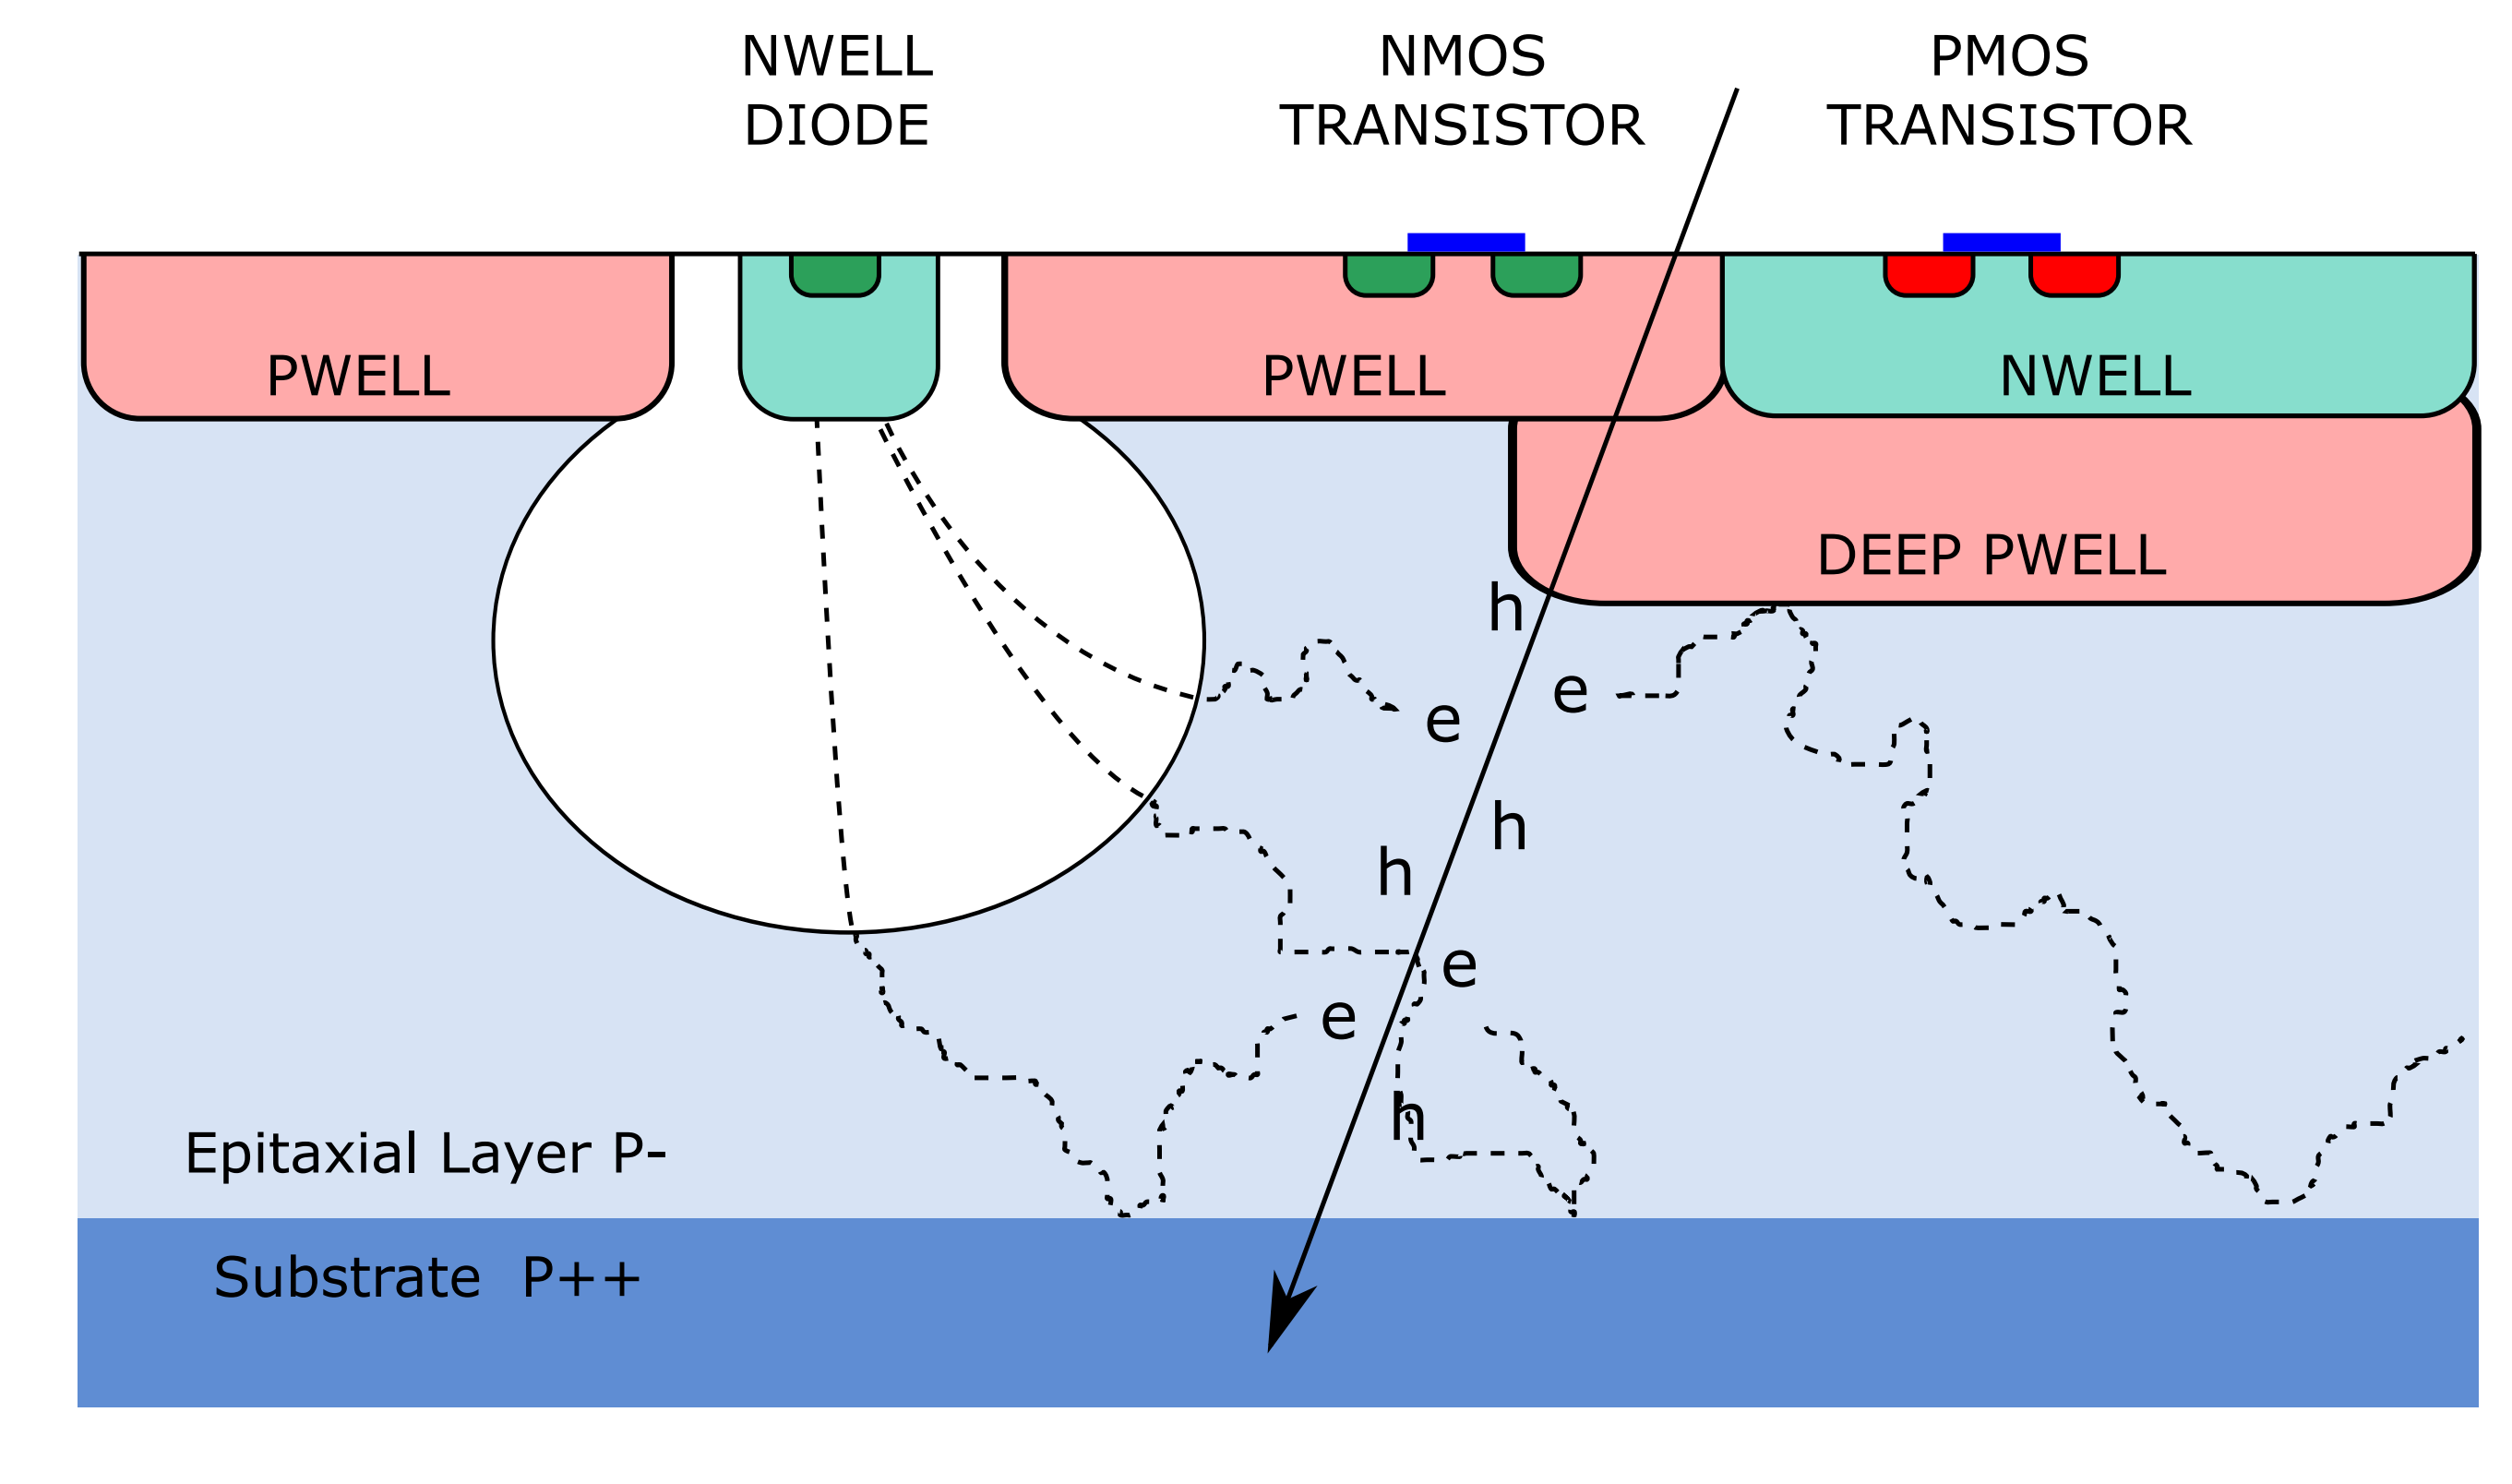
\includegraphics[width=0.8\textwidth]{figures/experiment/alpide_cross.png}
    \caption{A diagram showing the basic operating principle of a MAPS pixel.}
    \label{fig:alpide_diagram}
\end{figure}

These CMOS transistors work together to form the logic within the pixel, shown as a block diagram in Figure ~\ref{fig:alpide_l}. First, the collection diode sends a signal \textit{SUB}, which comes in the form of a large voltage drop in a very short ($\approx 10$ ns) time, followed by a slow requilibration. The \textit{VPULSE} signal is used for testing purposes, where a ``fake'' charge can be sent to the capacitor, generating a similar signal to the collection diode. The resulting \textit{PIX\_IN} signal is sent to an amplifier $+$ signal shaper, and then to a discriminator with threshold \textit{THR}. If the amplified signal is less than the threshold, no \textit{OUT\_D} signal is generated. The digital \textit{OUT\_D} signal is then sent into a simple AND gate, where the other input signal is the digital \textit{STROBE}. This strobing window is ultimately initialized by a trigger signal, and its width is configurable. If the \textit{OUT\_D} signal is high during the strobing window, then one of the three hit storage registers is ``latched'' (i.e. set to one). Also included in the pixel logic is a masking register, which masks the pixel during readout when hot. 

The priority encoder (which physically lies between two columns of pixels) sequentially provides the addresses of the latched pixels to the frontend electronics on the chip. An important feature of the on-pixel electronics and priority encoder is the lack of a clock: this means that there is no activity if there are no hits. In other words, the ALPIDE chip is not sending a bunch of useless 0's to the readout electronics, saving precious bandwidth.

\begin{figure}
    \centering
    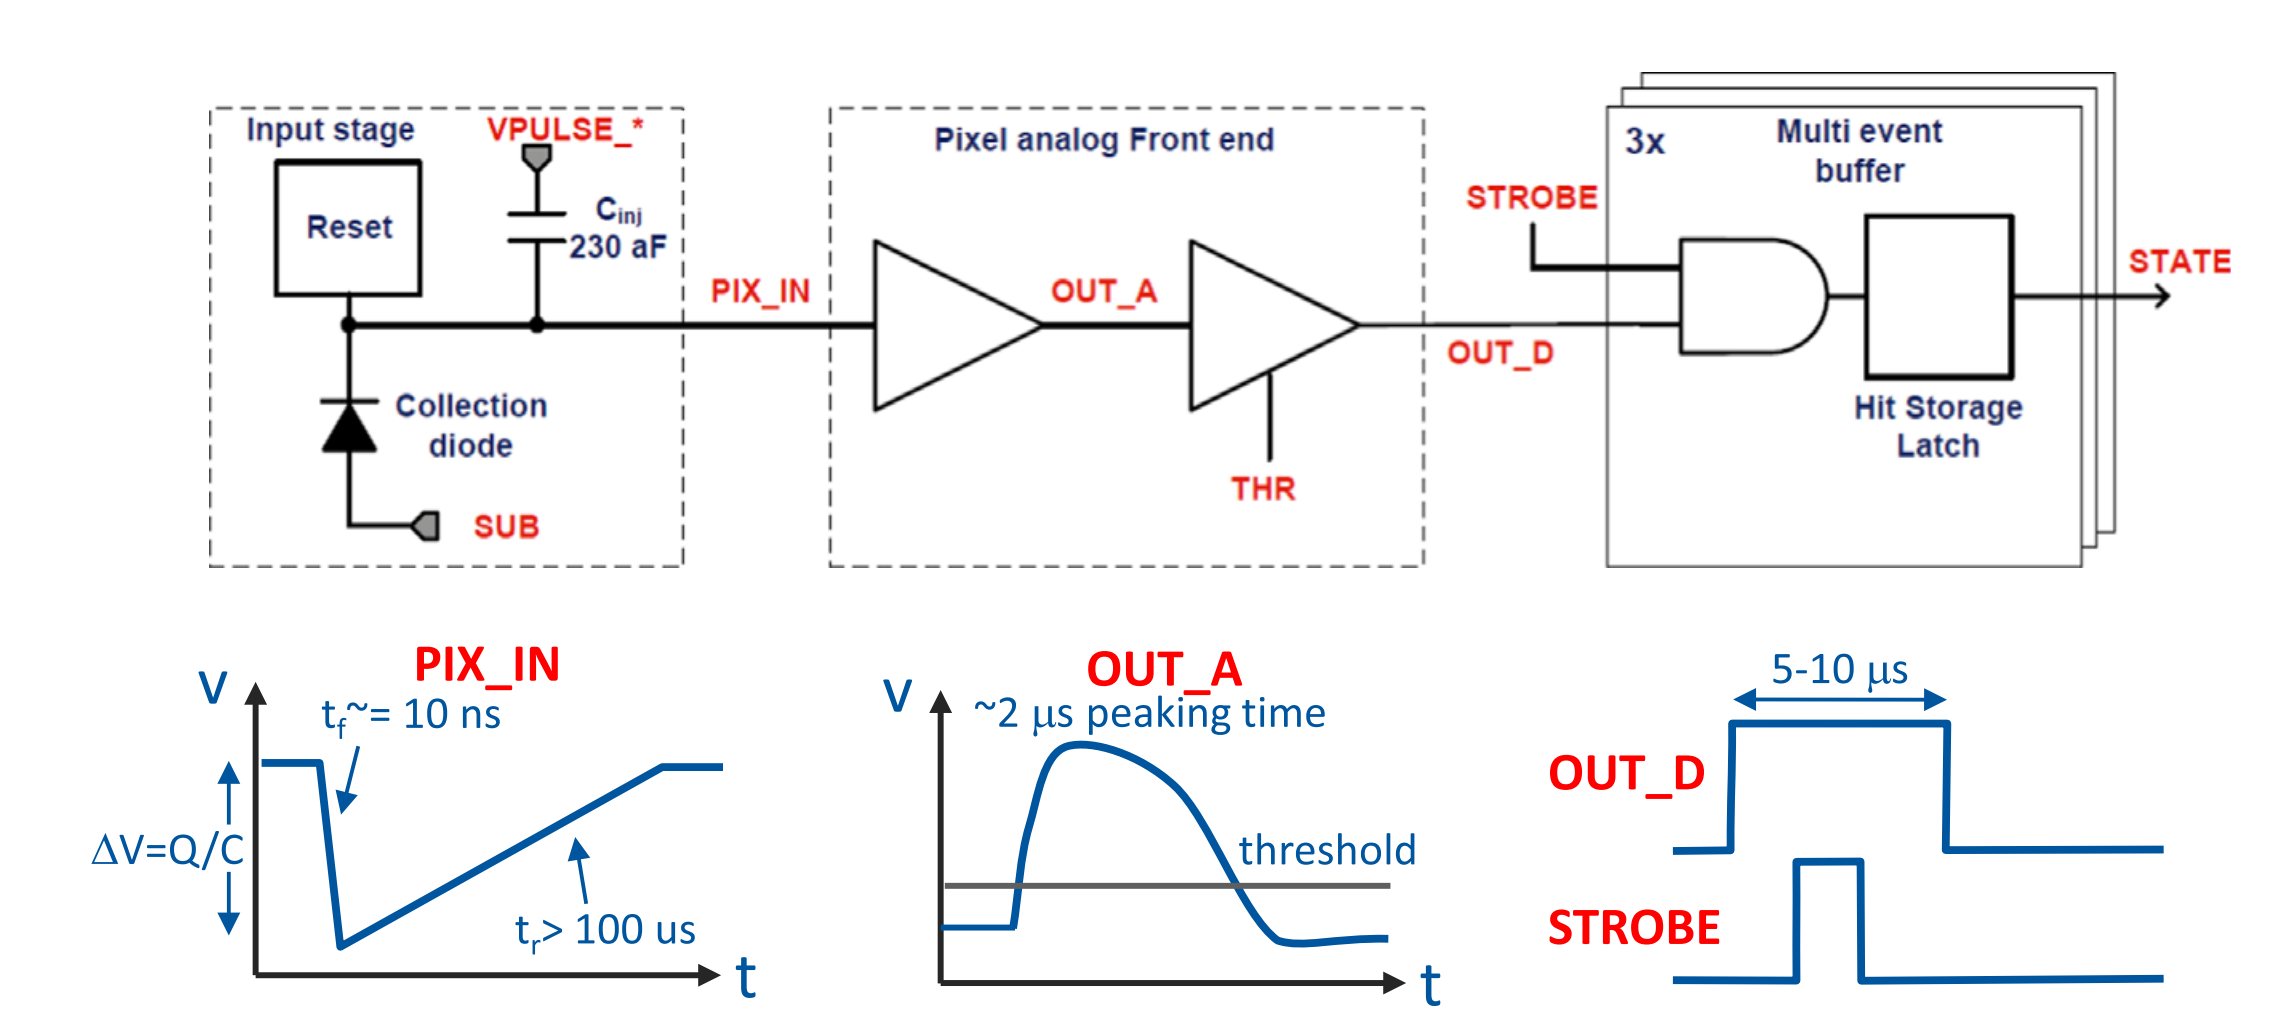
\includegraphics[width=1.0\textwidth]{figures/experiment/alpide_logic.png}
    \caption{A block diagram showing the logic embedded on top of a single ALPIDE pixel.}
    \label{fig:alpide_l}
\end{figure}

\subsubsection{Characterizing the chips for commissioning}
\label{sec:hardware_testing}

Each ALPIDE chip has over 500,000 pixels, each with their own circuit logic. Excluding issues with the frontend electronics on the chip, that is still \textit{over} 500,000 possible points of failure. As such, the chips were thoroughly tested to determine if they are worthy of being installed in the ITS. There are three main tests that were performed on each chip:
\begin{enumerate}
    \item \textbf{Fake hit rate}: All pixels are unmasked, and a \textit{STROBE} signal is repeatedly sent to each pixel. As the \textit{THR} signal should prevent any hits from being registered, any latched pixels are considered ``fake hits''.
    \item \textbf{Threshold scan}: A predetermined amount of charge is injected into each pixel via the \textit{VPULSE} signal, and the \textit{THR} signal is varied. There should be a clear threshold where every pixel registers a hit, and vice-versa.
    \item \textbf{Readout tests}: Either a digital signal (by writing the hit storage register) or an analog signal (by injecting charge into the capacitor) pattern is sent to the entire chip, and then the corresponding output is read out. The resulting output should be the same as the input, like the example shown in Figure~\ref{fig:ut_alpide}.
\end{enumerate}

\begin{figure}
    \centering
    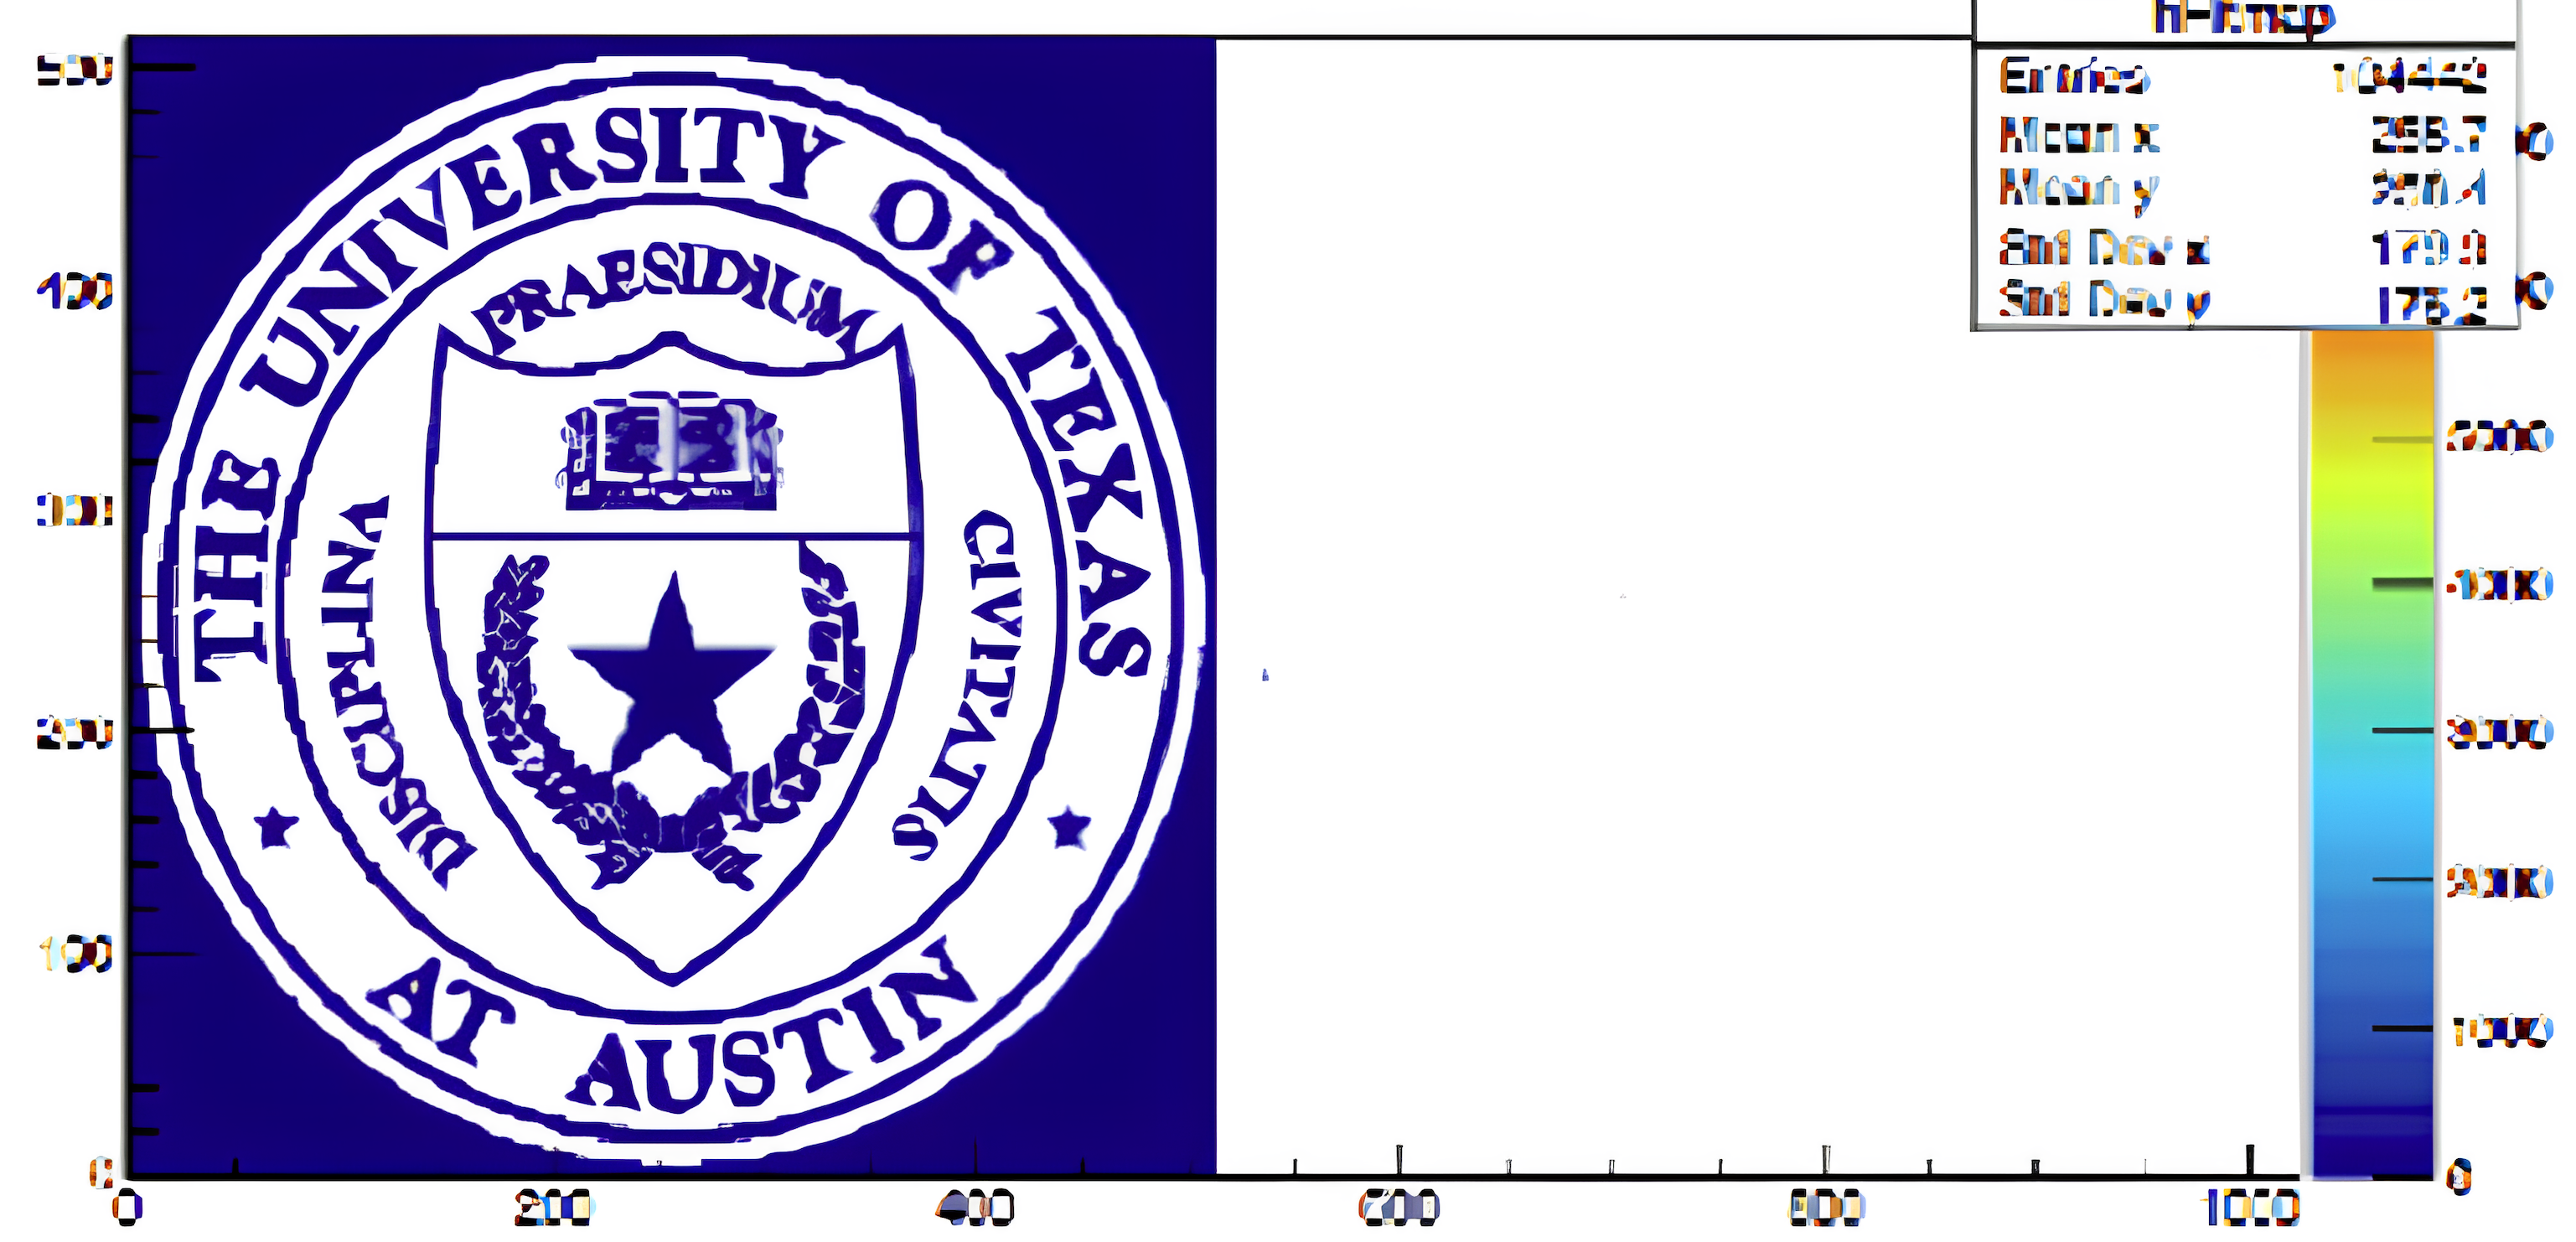
\includegraphics[width=0.9\textwidth]{figures/experiment/ut_alpide.png}
    \caption{The signal that was read out from the ALPIDE chip after sending an extremely technical digital input pattern.}
    \label{fig:ut_alpide}
\end{figure}

These tests were run on the ALPIDE software, which is a graphical user interface (GUI) that allows for easy communication with the chips. The resulting output of the tests was simply one of four options, which are summarized in Table~\ref{tab:chip_medals}. This medal system was used to determine where the chip should be installed within the detector. If a chip was GOLD, it was reserved for the IB. If the chip was SILVER, it could be installed in either the MLs or the OLs. If the chip was BRONZE, it could only be installed in the OLs. Finally, if the chip FAILed the tests, it was discarded\footnote{Sent to the poor souls developing the ALPIDE software.}. Further characterization was done at the stave level to determine where within the IB or OB a particular stave should be installed.

\begin{table}
    \centering
    \caption{A summary of the medal system used to determine where a particular chip should be installed. Note that while 99\% \textit{seems} strict, it corresponds to over 5000 misbehaving pixels.}
    \begin{tabular}{|c|c|}
        \hline
        \textbf{Medal} & \textbf{\% of good pixels} \\
        \hline
        GOLD & 99.99\% \\
        SILVER & 99.67\% \\
        BRONZE & 99.00\% \\
        FAIL &  $<$ 99.00\% \\
        \hline
    \end{tabular}
    \label{tab:chip_medals}
\end{table}

\subsubsection{The readout unit}
Another large overhaul for the ITS upgrade was a complete redesign of the readout system, from chip to DAQ. A schematic of the new readout system can be seen in Figure~\ref{fig:its_readout}. Each detector stave is connected to a \textbf{readout unit} (RU) via a relatively long copper data cable. A single RU has a lot of responsibilities, including
\begin{itemize}
    \item communicating with the power board so it can properly power the chips,
    \item receiving the trigger information from the Central Trigger Processor (CTP) and sending it to the chips (which generates the \textit{STROBE} signal discussed above),
    \item receiving \textit{all} of the data from the chips on the stave, which each have their own 1.2 Gbps link (for the IB chips, the OB chips share a 400 Mbps link in groups of seven), and
    \item sending the readout data from the chips to the Common Readout Unit (CRU), 
\end{itemize}
all while being in a highly radiative environment (only 6-8 meters away from the detector). 

\begin{figure}[h]
    \centering
    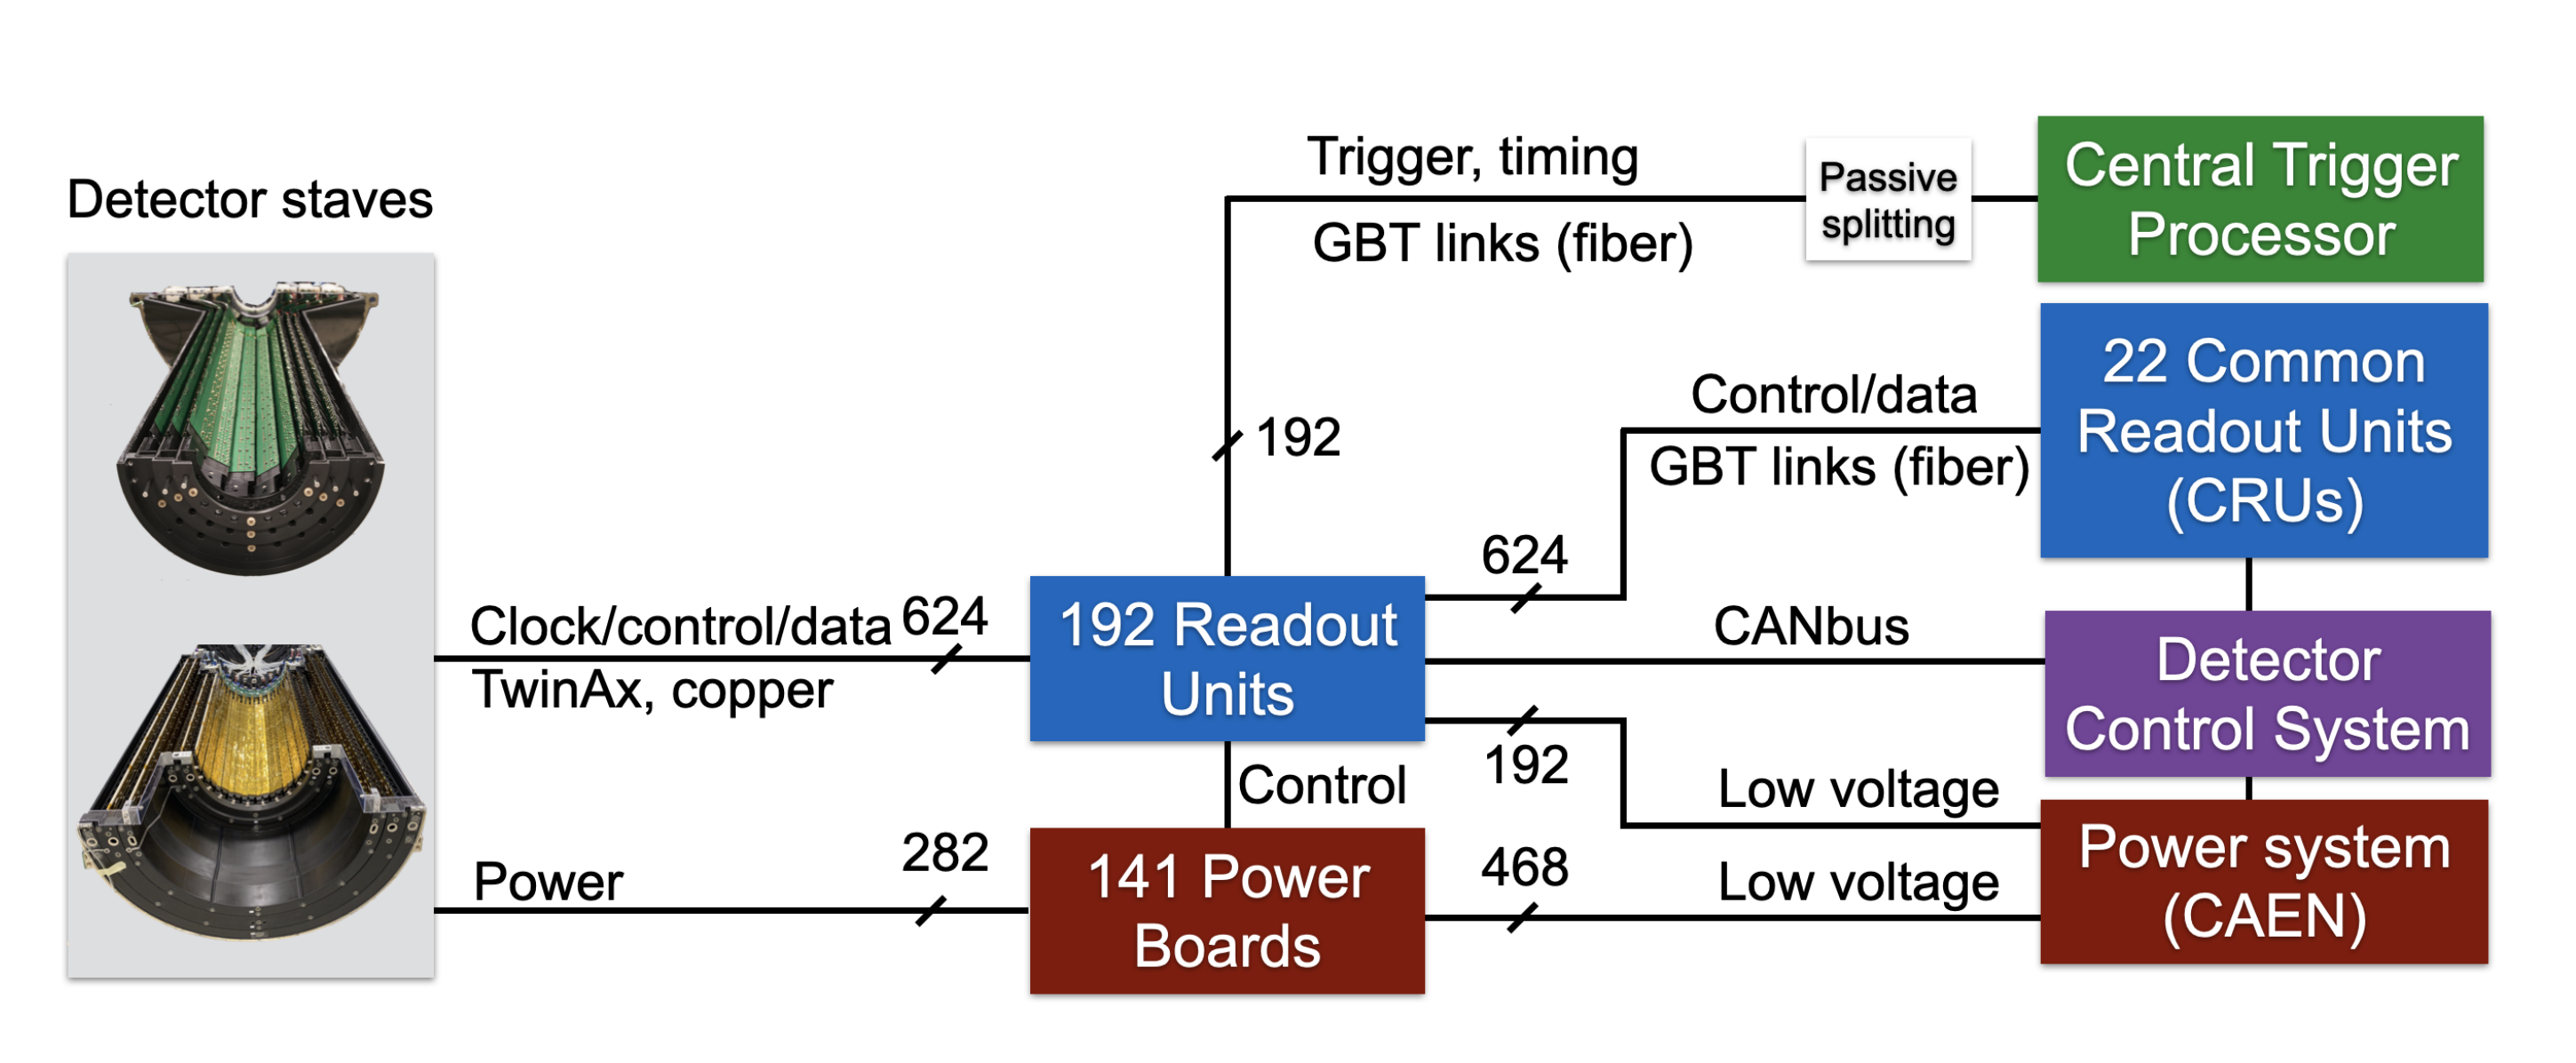
\includegraphics[width=0.9\textwidth]{figures/experiment/its_readout.png}
    \caption{A schematic of the ITS readout system, showing the various components of the system.}
    \label{fig:its_readout}
\end{figure}

These responsibilities are mostly handled by two on-board field-programmable gate arrays (FPGAs): an SRAM FPGA for actually handling all of the aforementioned data transfer between the various components, and a flash FPGA for ensuring that the SRAM FPGA does not misbehave in the radiative environment. The SRAM FPGA continuously scrubs the flash FPGA to ensure that it has not been misconfigured due to a radiation upset. If it has, the SRAM FPGA will reconfigure it using the ``golden image'' of the SRAM firmware stored in the flash memory of the flash FPGA (hence the name). Even still, the important modules of the SRAM FPGA are triplicated, meaning that if one module is subject to a radiation upset, the other two can outvote it. An image of the RU at the University of Texas at Austin can be seen in Figure~\ref{fig:ut_ru}.

\begin{figure}
    \centering
    \includegraphics[width=0.9\textwidth]{figures/experiment/ut_ru.png}
    \caption{A picture of a readout unit in its (not-so) natural habitat at the University of Texas at Austin. The heat sink and fan are covering the main SRAM FPGA, and to its north-east is the flash FPGA.}
    \label{fig:ut_ru}
\end{figure}

\section{The Time Projection Chamber}
\label{sec:tpc}
The largest component of the ALICE detector is known as the Time Projection Chamber (TPC)~\cite{TPC1, TPC2}. The TPC is a gas-filled volume with an 85 cm inner radius, a 250 cm outer radius, and a five meter length along the beam axis. This corresponds to an active volume of around 90 cubic meters, all of which is filled with a Ne-CO$_2$-N$_2$ (90-10-5) gas mixture. The TPC has The TPC is an ionizing drift detector: charged particles moving through the detector ionize the gas, and the resulting electrons drift towards the endplates of the detector\footnote{A very similar mechanism to the SDD, on a much larger scale.}--heavily coerced by the presence of a strong 400 V/cm electric field along the z-axis. This electric field is generated by a central cathode that is kept at a potential of 100 kV. A schematic of the TPC field cage can be seen in Figure~\ref{fig:tpc_schematic}.

\begin{figure}
    \centering
    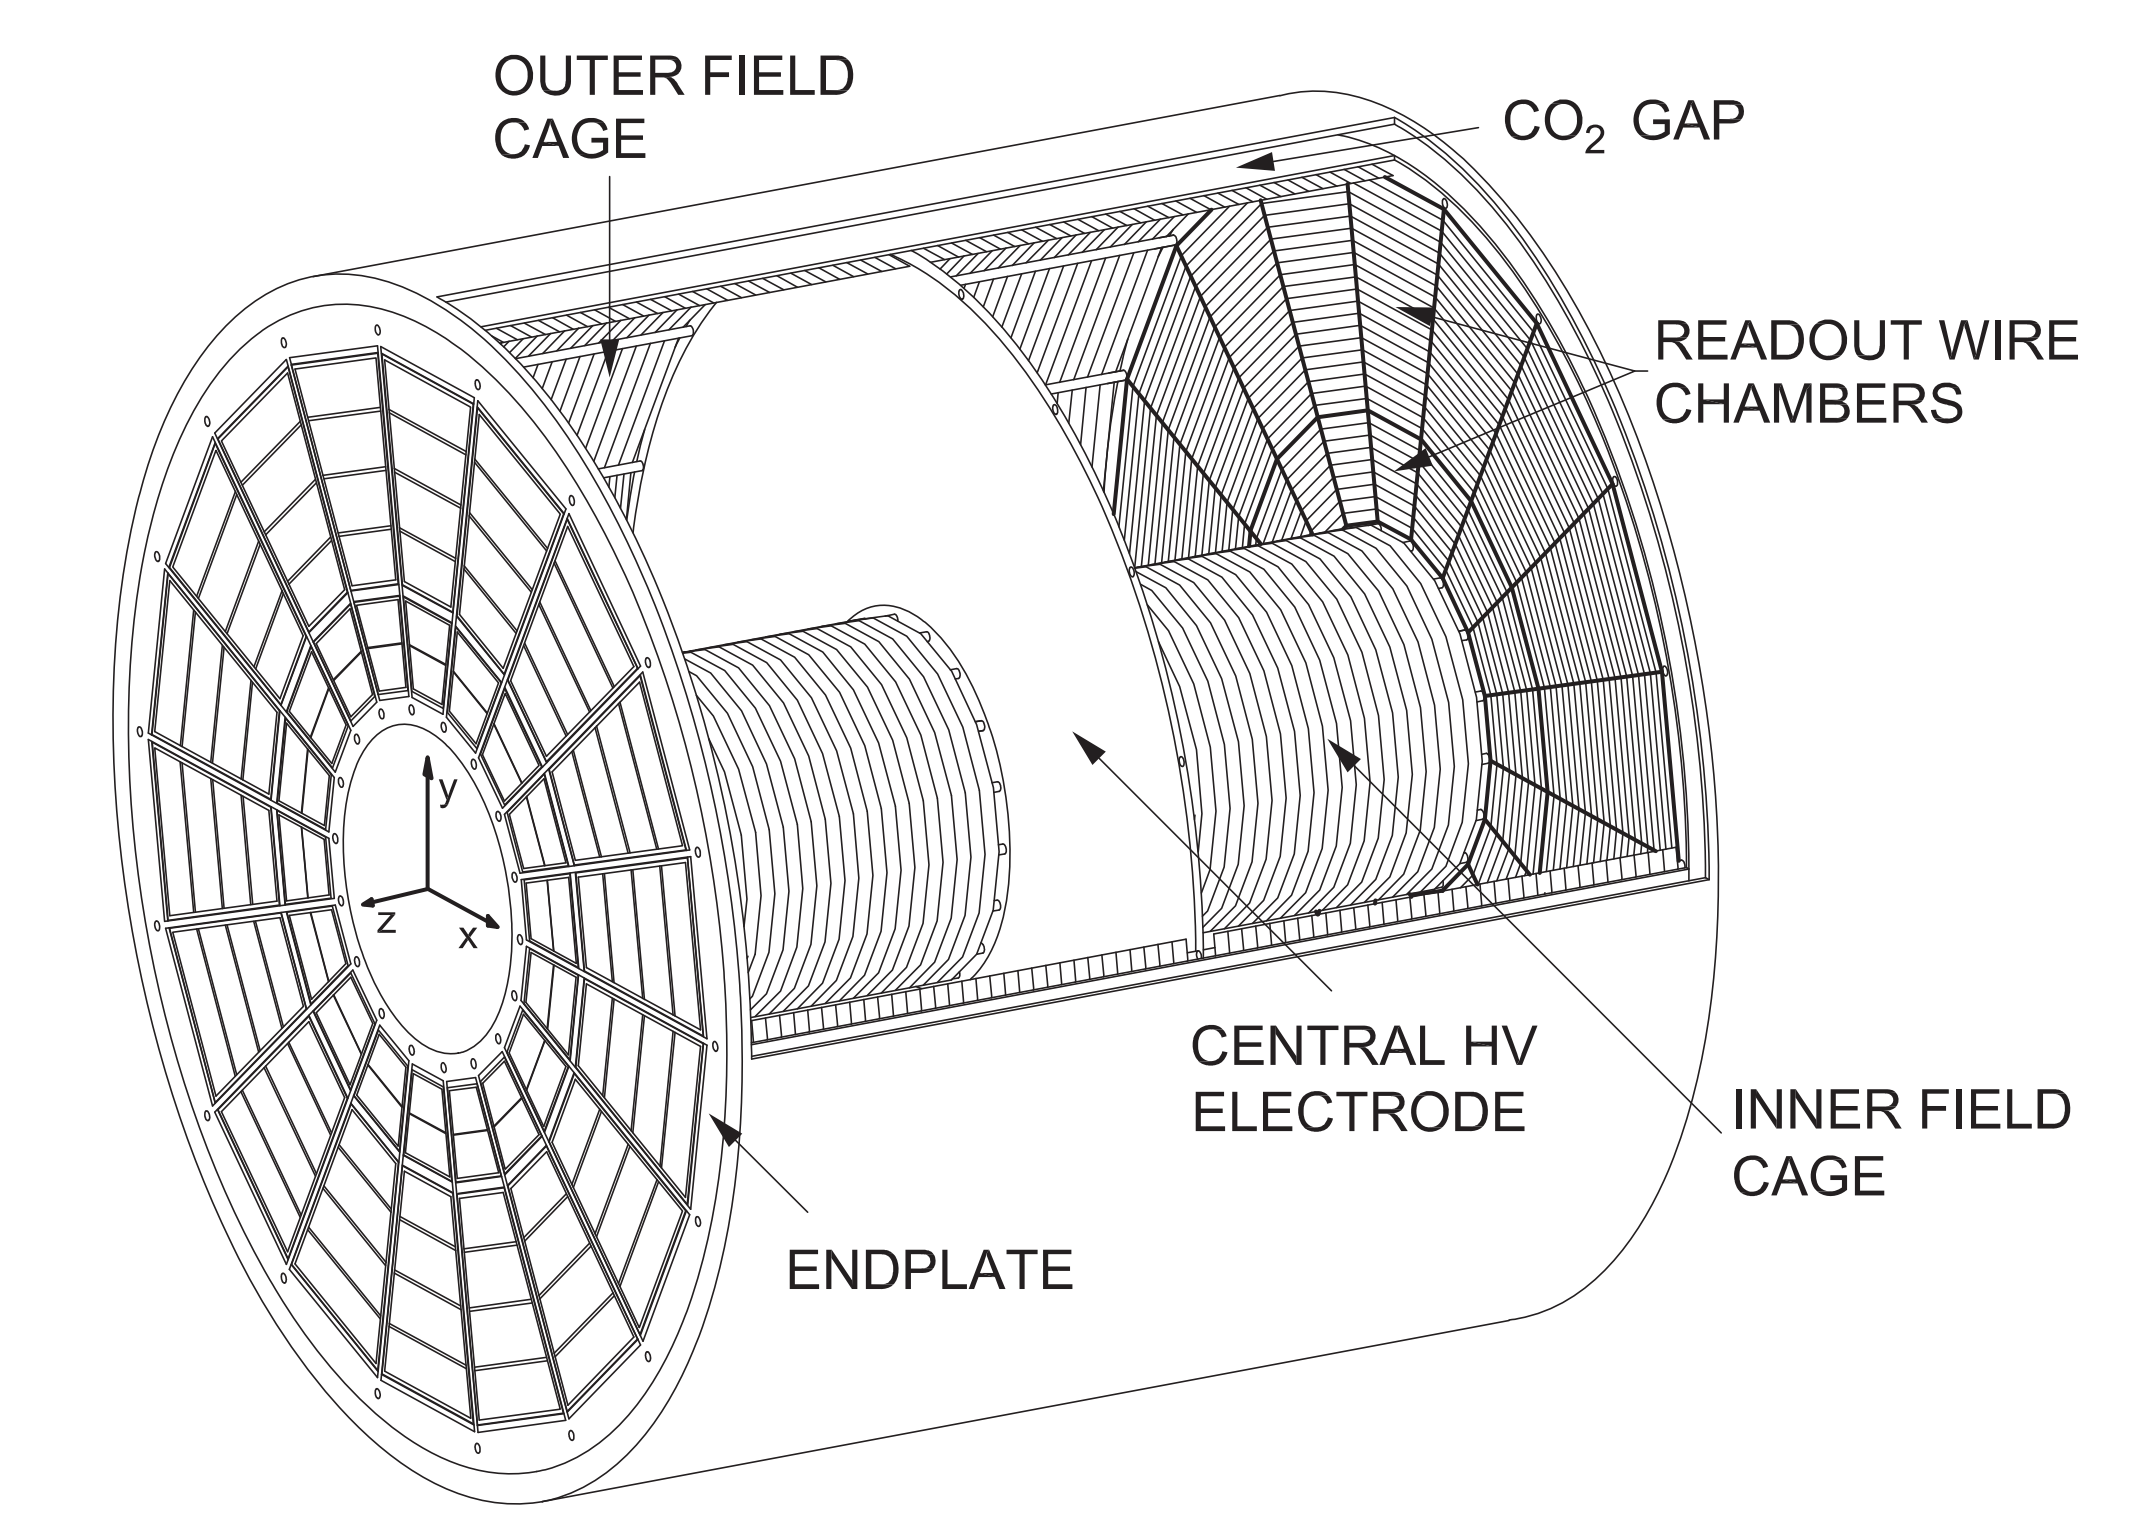
\includegraphics[width=0.9\textwidth]{figures/experiment/tpc_schematic.png}
    \caption{A schematic of the TPC field cage, taken from~\cite{TPC1}}
    \label{fig:tpc_schematic}
\end{figure}

Readout chambers with design based off of the Multi-Wire Proportional Chamber (MWPC) technique are installed at both endplates. In short, these chambers contain an array of wires held at a high voltage are placed in front of a plane of pads held at ground. The electrons that drift towards the endplate pass through this region, which causes a localized cascade of ionization\footnote{Often called a Townsend avalanche, where the ionizing electrons from the initial ionization of the ionizable gas ionize the ionizable gas, creating more ionizing electrons to ionize more ionizable gas...} that is ultimately collected by the pads. The inner readout chamber has 5504 total pads, while the outer readout chamber (i.e. the one actually visible in Figure~\ref{fig:tpc_schematic}) has nearly 10000. The pads are grouped into 18 trapezoidal sectors, each of which covers 20$^\circ$ in azimuth. Unfortunately the boundaries of these sectors don't contain any pads, resulting in very narrow ``dead zones'' within the azimuthal acceptance of the TPC. Using information from both the ITS and TPC, it is possible to reconstruct particle tracks with a resolution of 1 mm in the transverse plane and 2 mm in the longitudinal direction. The momentum resolution in the transverse plane is also very good, staying below 5\% from zero to well over 100 GeV/c.

The TPC is also capable of providing information that can be used to identify particles. As a charged particle travels through the active volume of the TPC, it loses energy as it ionizes the gas in a way that only depends on the particle's velocity. This energy loss is often described by the Bethe-Bloch formula~\cite{BetheBlochPDG}
\begin{equation}
    \left\langle-\frac{d E}{d x}\right\rangle=K z^2 \frac{Z}{A} \frac{1}{\beta^2}\left[\ln \frac{2 m_e c^2 \beta^2 \gamma^2}{I}-\beta^2-\frac{\delta(\beta \gamma)}{2}\right]
\end{equation}
where $K$ is a constant coefficient ($\approx 0.31$ MeV mol$^{-1}$ cm$^2$), $z$ is the charge of the particle, $Z$ and $A$ are the atomic and mass numbers of the gas, $\beta$ is the velocity of the particle in units of the speed of light, $\gamma$ is the Lorentz factor, $m_e$ is the mass of the electron, $c$ is the speed of light, and $I$ is the mean excitation energy of the gas. An important feature of this equation is that most of the parameters depend on the gas mixture and the mass of the electron. For a fixed gas mixture, this equation gives a relationship between the energy (loss) and the velocity of the particle. As the momentum of the particle is known, the mass (and therefore the particle species) can be determined. To see this explicitly, it is useful to look at a common parameterization of the Bethe-Bloch formula~\cite{BetheBlochALEPH},
\begin{equation}
    f(\beta \gamma)=\frac{P_1}{\beta^{P_4}}\left(P_2-\beta^{P_4}-\ln \left(P_3+\frac{1}{(\beta \gamma)^{P_5}}\right)\right),
\end{equation}
where parameters $P_i$ only depend on the gas mixture. Rewriting this equation in terms of the momentum $p$ of the particle gives a curve for each particle species with mass $m_i$,
\begin{equation}
    \label{eq:bethe_bloch_par}
    f(p, m_i)= P_1 \left(\frac{\sqrt{m_i^2 + p^2}}{p}\right)^{P_4} \left(P_2 - \left(\frac{p}{\sqrt{m_i^2 + p^2}}\right)^{P_4}  - \ln \left(P_3 + \frac{m_i^{P_5}}{p^{P_5}} \right) \right).
\end{equation}

\begin{figure}
    \centering
    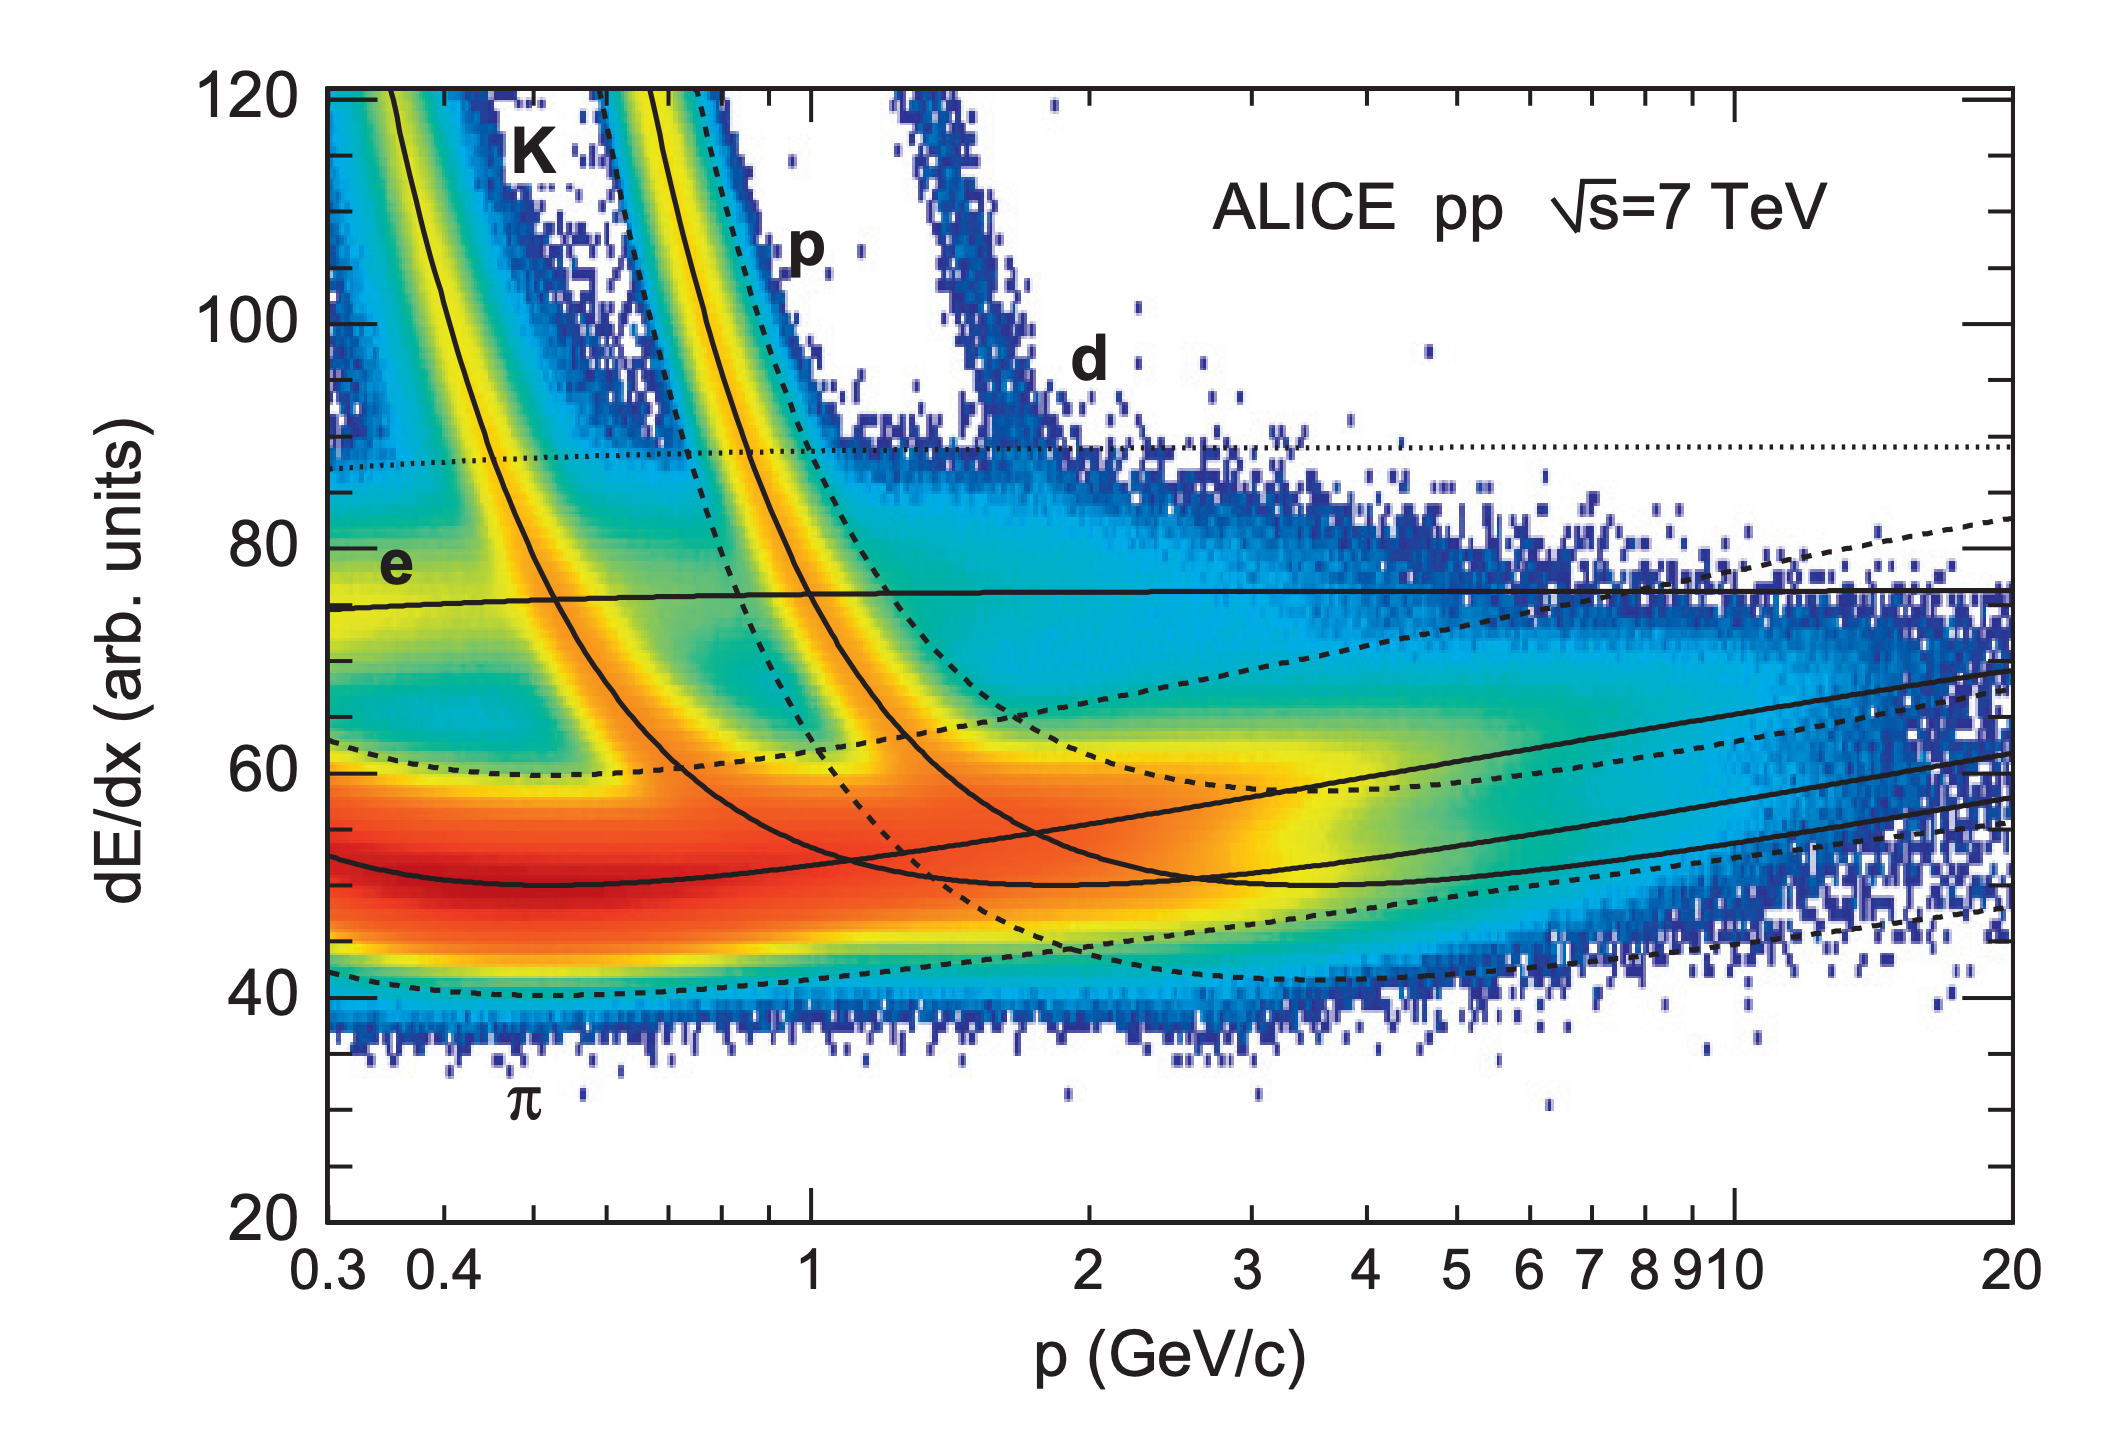
\includegraphics[width=0.9\textwidth]{figures/experiment/tpc_pid_curves.png}
    \caption{The energy loss signal for different particle species using the ALICE TPC gas mixture, taken from~\cite{BetheBlochALEPH}. The solid lines represent the expected energy loss signal for each particle species (Equation~\ref{eq:bethe_bloch_par}).}
    \label{fig:tpc_pid_curves}
\end{figure}

Examples of the energy loss signal for different particle species using the ALICE TPC gas mixture can be seen in Figure~\ref{fig:tpc_pid_curves}. Note that while there are clearly defined lines for each particle species from Equation~\ref{eq:bethe_bloch_par}, the actual signal is spread out around these lines due to the energy loss and momentum resolution of the TPC. Furthermore, many of the curves intersect at higher momentum. As such, it is useful to define the quantity 
\begin{equation}
n\sigma_{\text{TPC}} = \frac{\langle dE/dx \rangle_{\text{meas}} - \langle dE/dx \rangle_{\text{exp}}}{\sigma_{\text{TPC}}},
\end{equation}
which is the number of standard deviations away from the expected energy loss signal for a given particle species. If an unidentified particle has an $n\sigma_{\text{TPC}}$ value close to zero, it is likely that the particle is of that species. However, when investigating a specific particle species, compromises must be made--requiring a low $n\sigma_{\text{TPC}}$ value may result in less contamination from other particle species, but also yields lower statistics.

\section{The Time of Flight detector}
\label{sec:tof}

The Time of Flight (TOF) detector~\cite{TOF1} is a large array of Multi-gap Resistive Plate Chambers (MRPCs)~\cite{TOF2} that is used to measure the time of flight of charged particles from the nominal interaction point. The TOF is located directly outside of the TPC at a radius of around 3.7 meters, and covers the pseudorapidity range $|\eta| < 0.9$. It consists of 1593 MRPC strips, arranged in 18 sectors along the azimuthal direction. Each MRPC strip has two rows of 48 pickup pads with area 3.5 $\times$ 2.5 cm$^2$, to ensure low occupancy even in the most crowded events. This gives a total of 96 pads per strip and 152928 readout channels in total. The TOF MRPC has a double-stack structure; each of the two stacks has five gas gaps each. The resistive plates are made of standard soda-lime glass sheets. The gap (250 µm) is created by commercial fishing line stretched over the glass sheets. The average MRPC time resolution, including the effects of the full front-end and readout electronics, was measured to be better than 50 ps in a beam test setup.

\begin{figure}
    \centering
    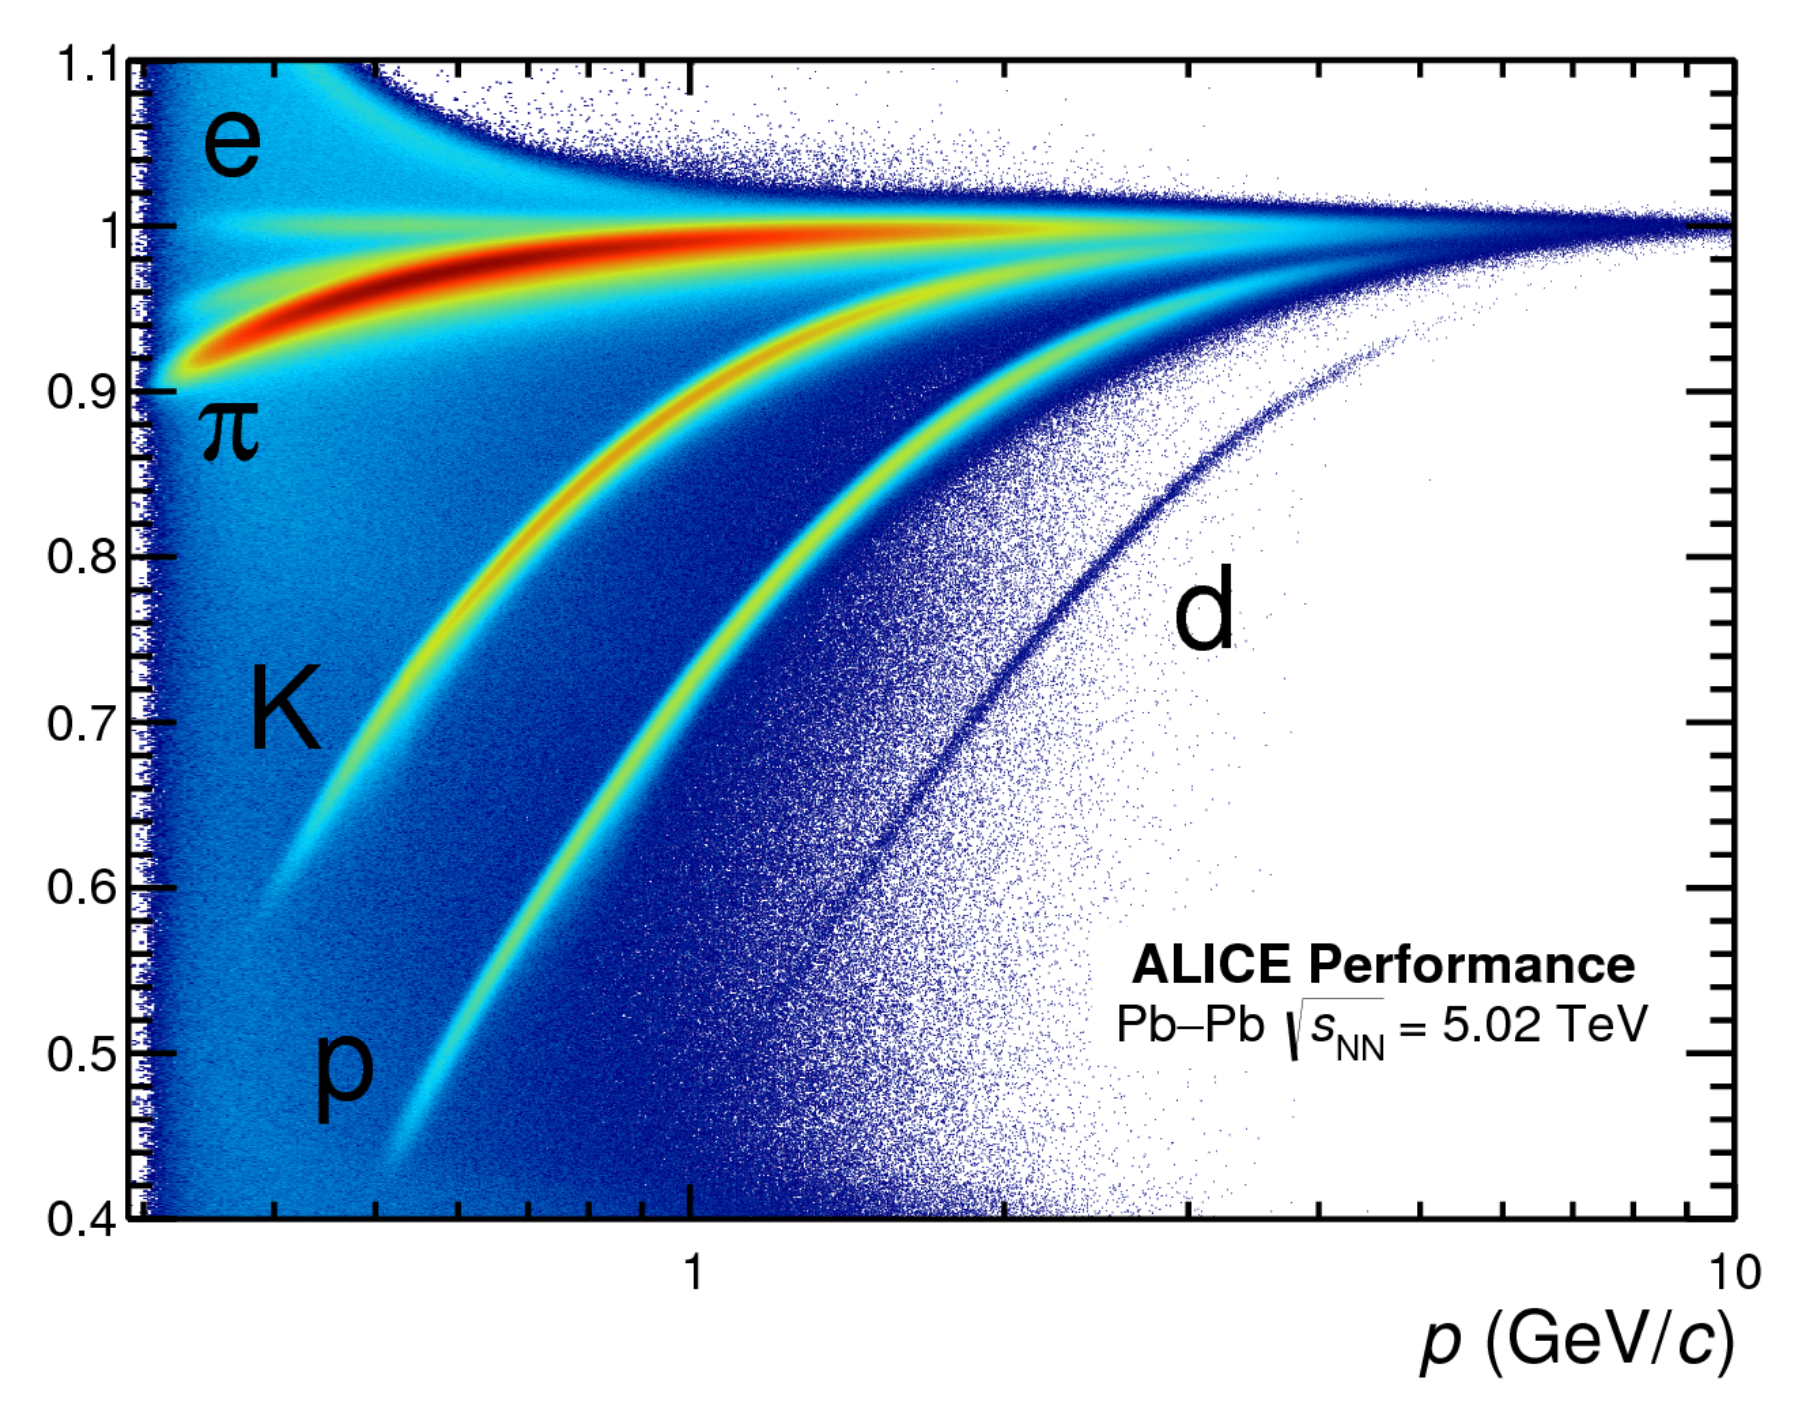
\includegraphics[width=0.9\textwidth]{figures/experiment/tof_pid_curves.png}
    \caption{The time of flight signal $\beta_{\text{TOF}}$ measured in 5.02 TeV Pb--Pb collisions for different particle species as a function of momentum~\cite{TOFPIDPlot}. The curves are labeled with the particle species they correspond to.}
    \label{fig:tof_pid_curves}
\end{figure}

The primary goal of the TOF detector is particle identification: the time of flight of a particle is directly related to its velocity (as the TOF is a fixed length away from the interaction point), which can be used with the particle's momentum to determine its mass. More explicitly, the velocity $\beta$ of a particle is given by (in natural units)
\begin{equation}
    \beta_{\text{TOF}} = \frac{L}{t_{\text{TOF}}},
\end{equation}
where $L$ is the distance from the interaction point to the TOF (3.7 meters) and $t_{\text{TOF}}$ is the time of flight of the particle. Using $p =  m \frac{\beta}{\sqrt{1-\beta^2}}$, $\beta_{\text{TOF}}$ can be written as a function of $p$ for a particle of mass $m_i$,
\begin{equation}
    \beta_{\text{TOF}}(p, m_i) = \frac{p}{\sqrt{p^2 + m_i^2}}.
\end{equation}
Much like the TPC, plotting the TOF signal versus momentum provides a unique curve for each particle species, as shown in Figure~\ref{fig:tof_pid_curves}. Also much like the TPC, the signal is spread out around the expected curve due to the timing resolution of the TOF and momentum resolution of the TPC $+$ ITS. As such, the quantity
\begin{equation}
n\sigma_{\text{TOF}} = \frac{\beta_{\text{meas}} - \beta_{\text{exp}}}{\sigma_{\text{TOF}}},
\end{equation}
is defined, which serves a similar purpose to $n\sigma_{\text{TPC}}$.



\section{The Electromagnetic Calorimeter}

The Electromagnetic Calorimeter (EMCal)~\cite{EMCAL1, EMCAL2} is a sampling calorimeter that consists of lead and polystyrene scintillator layers. The EMCal is made of towers, which are stacks of 76 lead layers (1.44 mm thick) and 77 polystyrene layers (1.76 mm thick). Each tower has a size of about 6.0 $\times$ 6.0 $\times$ 24.6 cm$^3$ and has an individual readout. The towers are arranged into 2 $\times$ 2 groups called modules, which are the smallest units of the detector. The modules are further assembled into larger supermodules (12 $\times$ 24 modules), each weighing about 7.7 metric tons. The EMCal has a total of 10 full-size supermodules and 2 one-third size supermodules, corresponding to 3072 modules and 12,288 towers. It covers a pseudorapidity range of $|\eta| < 0.7$ and an azimuthal angle range of  $\Delta\varphi = 107^\circ$. It is positioned around 4.5 meters from the beam line, between the space-frame support structure and the L3 magnet coils. Schematics of the detector components can be seen in Figure~\ref{fig:emcal_schematic}. While not used in this thesis, the University of Texas at Austin was involved in the commissioning of the EMCal, and thus it is worth mentioning for historical purposes.

\begin{figure}
    \centering
    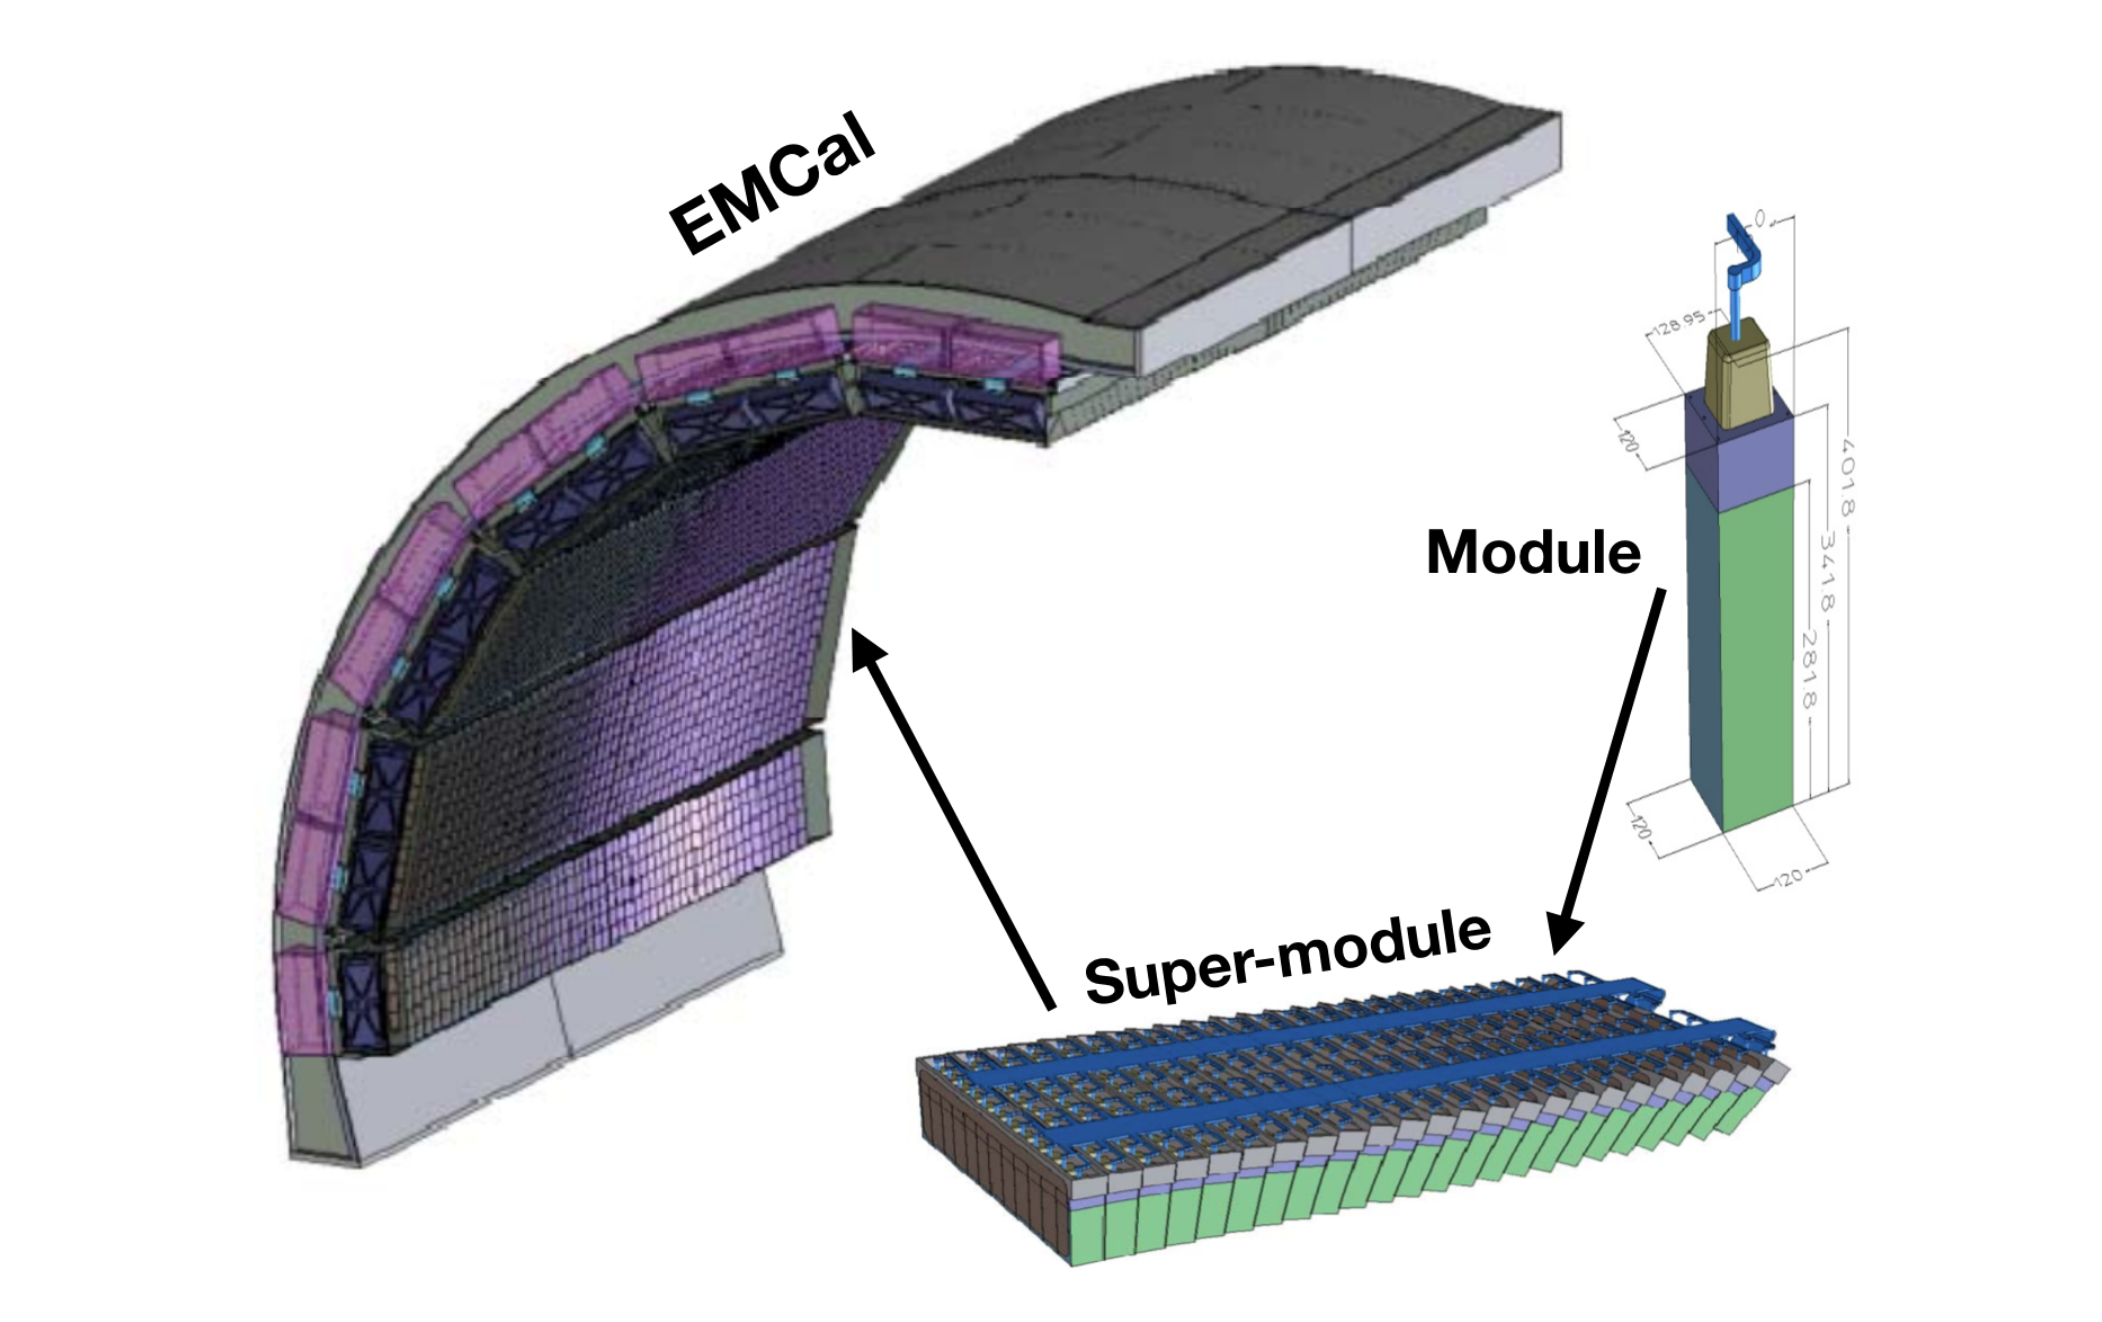
\includegraphics[width=0.9\textwidth]{figures/experiment/emcal_schematic.png}
    \caption{A schematic of the EMCal~\cite{ERIN123}, along with the module and supermodule structure~\cite{ERIN124}.}
    \label{fig:emcal_schematic}
\end{figure}

\section{The VZERO Detector}

The VZERO detector~\cite{VZERO} consists of two end-cap scintillators: the V0A, located in the forward pseudorapidity region ($2.8 < \eta < 5.1$); and the V0C, located in the backward region ($-3.7 < \eta < -1.7$). While most of the interesting physics lies at midrapidity, these detectors are vital for estimating the collision centrality (as discussed in Section~\ref{sec:collision_centrality}). The VZERO detectors also provide a trigger for the other detectors: whenever a coincident signal occurs in the V0A and V0C, a collision event must have occured between the two detectors. The VZERO system is also used to monitor LHC beam conditions and reject beam-gas and beam-halo events. As the data analyzed in this thesis is from p--Pb collisions, only information from the V0A detector--which faces the lead ion beam--is used for determining the multiplicity percentile of the collision events.